\documentclass[12pt,twoside]{report}   % or 11 pt if you're desperate for space.
\usepackage{amsmath, amssymb, amsthm, pgf, tikz}
\usepackage{graphicx, microtype, hyperref}
\usetikzlibrary{positioning,shapes,arrows}
\usepackage{fancyhdr}
\usepackage[toc,page]{appendix}
\usepackage{bm}
\usepackage{dcolumn}
\usepackage{booktabs}
\usepackage[labelfont=bf]{caption}
\usepackage{subcaption}
\usepackage{float}
\usepackage{parskip}
\usepackage{listings}
\usepackage[utf8]{inputenc}
\usepackage{color}
\usepackage{tcolorbox}
\definecolor{codeblue}{rgb}{0.12, 0.56, 1.0}
%\definecolor{codegreen}{rgb}{0.3,0.73,0.09}
\definecolor{codegrey}{rgb}{0.95,0.95,0.95}
%\definecolor{codeorange}{rgb}{0.93, 0.53, 0.18}
%\definecolor{codewhite}{rgb}{0.97, 0.97, 1.0}
\definecolor{backcolour}{rgb}{0.15, 0.15, 0.15}
\lstdefinestyle{mystyle}{
    backgroundcolor=\color{codegrey},   
%    commentstyle=\color{codegreen},
%    keywordstyle=\color{codeblue},
    numberstyle=\tiny\color{backcolour},
%    stringstyle=\color{codeorange},
%    basicstyle=\small\color{codewhite},
    breakatwhitespace=false,         
    breaklines=true,                 
    captionpos=b,                    
    keepspaces=true,                 
    numbers=left,                    
    numbersep=5pt,                  
    showspaces=false,                
    showstringspaces=false,
    showtabs=false,                  
    tabsize=2
}

\newcounter{nalg}[chapter] % defines algorithm counter for chapter-level
\renewcommand{\thenalg}{\thechapter .\arabic{nalg}} %defines appearance of the algorithm counter
\DeclareCaptionLabelFormat{algocaption}{Pseudocode \thenalg} % defines a new caption label as Algorithm x.y

\lstnewenvironment{Pseudocode}[1][] %defines the algorithm listing environment
{   
    \refstepcounter{nalg} %increments algorithm number
    \captionsetup{labelformat=algocaption,labelsep=colon} %defines the caption setup for: it ises label format as the declared caption label above and makes label and caption text to be separated by a ':'
    \lstset{ %this is the stype
    	backgroundcolor=\color{codegrey},
    	numberstyle=\tiny\color{backcolour},
    	numbersep=5pt,
        tabsize=2,
        frame=tB,
        numbers=left, 
        keywordstyle=\color{codeblue}\bfseries,
        keywords={,input, output, return, datatype, function, in, if, else, foreach, while, begin, end, } %add the keywords you want, or load a language as Rubens explains in his comment above.
        numbers=left,
        xleftmargin=.04\textwidth,
        #1 % this is to add specific settings to an usage of this environment (for instnce, the caption and referable label)
    }
}
{}
\hypersetup{
    colorlinks=true,
    citecolor=red,
    linkcolor=blue,
    filecolor=blue,      
    urlcolor=blue,
}
 
%\lstset{style=mystyle}
\def\ContinueLineNumber{\lstset{firstnumber=last}}
\def\StartLineAt#1{\lstset{firstnumber=#1}}
\let\numberLineAt\StartLineAt
%%%%%%%%%%%%%%%%%%%%%%%%%%%%%
\newcommand{\bkt}[1]{\left( #1 \right)}
\newcommand\aap{}
\newcommand{\bb}{\textbf}
\newcommand{\ti}{\textit}
\newcommand{\R}{\mathbb{R}}
\newcommand{\N}{\mathbb{N}}
\newcommand{\p}{\prime}
\newcommand{\te}{\text}

\DeclareMathOperator*{\argmax}{arg\,max}

\newtheorem{theorem}{Theorem}[section]
\newtheorem{maintheorem}[theorem]{Main Theorem}
\newtheorem{definition}[theorem]{Definition}
\newtheorem{lemma}[theorem]{Lemma}
\newtheorem{proposition}[theorem]{Proposition}
\newtheorem{corollary}[theorem]{Corollary}


%%%%%%%%%%%%%%%%%%%%%%%
% This stuff below sets the page layout. Don't change these.
\addtolength{\topmargin}{-2.7cm}
\addtolength{\textheight}{5cm}
\setlength{\headheight}{15pt}
\evensidemargin 14pt
\oddsidemargin 14pt
\textwidth 6.2in
\raggedbottom
\widowpenalty=5000
\clubpenalty=1000

%%%%%%%%%%%%%%%%%%%%%%%

\newcolumntype{M}[1]{D{.}{.}{1.#1}}

\begin{document}


\begin{titlepage}
    \begin{center}
        \vspace*{1cm}
        
        \Huge
        \textbf{Markov Chain Monte Carlo Sampling Algorithms \& Machine Learning Applications}
        
        \vspace{0.5cm}
        \LARGE
        Student Number 201503311
        
        \vspace{1.5cm}
        
        \textbf{Michael G. Turner}
        
        \vfill
        
        A thesis presented for the degree of\\
        Masters in Mathematics
        
        \vspace{0.8cm}
        
        \includegraphics[width=0.4\textwidth]{HullShield.pdf}
        
        \Large
        School of Mathematical \& Physical Sciences\\
        University of Hull\\
        United Kingdom\\
        $3^{\text{rd}}$ of May 2019
        
    \end{center}
\end{titlepage}

\thispagestyle{plain}
\begin{center}
    \Large
    \textbf{Markov Chain Monte Carlo Sampling Algorithms \& Machine Learning Applications}
    
    \vspace{0.4cm}
    \large
    Student Number 201503311
    
    \vspace{0.4cm}
    \textbf{Michael G. Turner}
    
    \vspace{0.9cm}
    \textbf{Abstract}
\end{center}

This report will go through the mathematics that are used in different computational random sampling methods known as Markov Chain Monte Carlo sampling algorithms or MCMC. I will present how these algorithms are implemented in the programming language R with different examples that will visualise how these algorithms work. I will discuss the work I have done into how machine learning classification works and go through some examples of different applications where they are used through another programming language Python. Now, without further ado, we shall begin.

\tableofcontents

\pagestyle{fancy}
\renewcommand{\chaptermark}[1]{ \markboth{#1}{} }
\renewcommand{\sectionmark}[1]{ \markright{#1}{} }
\fancyfoot{}
\fancyhead[RO,LE]{\thepage}
\fancyhead[RE]{MCMC Sampling Algorithms \& ML Applications}
\fancyhead[LO]{\leftmark}
\chapter{Introduction}\label{Intro}

Before diving into the details of computational random sampling methods I would like to go over some of the basic statistics you will need to understand what will be covered throughout this entire report. 

\section{The Frequentist Vs The Bayesian}\label{The F Vs B}
\vspace{-0.4in}
\underline{\hspace{6.2in}}
\vspace{-0.1in}

The very first thing to clarify is how Bayesian is different from Frequentist. The Frequentist views probability as being the \textit{relative frequency} of an event occurring in an infinitively long series of \textit{identical} trials. This can be represented in a mathematical expression as
\begin{align*}
P(h) = \lim_{n\to\infty} \frac{h}{n}
\end{align*}
where $h$ is the number of times that the event occurred and $n$ is the total number of trials. This might appear perfectly logical but the trouble lies in the assumptions, one of which says that the trials are \ti{identical}. This is bad news because, in the real world, the different variables will not be identical each time we flip the coin.

Suppose that I flipped a coin at $67.3$cm from the ground and the coin had an orientation to the ground that was an angle of $32^{\circ}$ relative to the horizontal and $2^{\circ}$ relative to the vertical. If I repeated this set up \textit{exactly} then I should expect to get a certain value out with every flip because the system is in itself deterministic, right? This is where we encounter issues with the Frequentist view with what is truly meant by the term \ti{identical}.

We could possibly determine the coin to be a set height from the ground but allow the orientation to alter, but then we start to enter a subjective view for what identical means which goes against the Frequentist belief. For a real life scenario like this there is always going to be a sense of uncertainty because the experiment cannot be recreated exactly as before. With a Bayesian perspective, we can avoid this issue.

For Bayesian, we think of the probability of an event occurring as the number of events divided by the number of possible outcomes, which are all to be \textit{equally} likely. What this means is that we could quantify all the possible orientations of the coin, which will be the \text{initial} conditions, and then look at the forces acting on the coin. We can combine these and then think about, for each of these conditions, what value will the coin give? So the number of possibilities is given by the number of initial conditions and the number of heads represents the total number of heads we get across all these different possibilities.

Like with the Frequentist approach, there are some assumptions being made here as well which is that the data is fixed. What that would mean is that, given some initial condition like the orientation and height of the coin, we would get the same value every time. But the reason we do not is because the parameters can vary.

This is much more realistic approach as the Bayesian probability does not represent a long run frequency of getting a head but rather an uncertainty. We do not know the exact initial orientation of the coin so we are left with some underlying uncertainty with whether we will get a head or a tails.

It could be regarded as common sense to know that you can never be \textit{completely} certain of an event happening. And it is also important that the Bayesian view does not rely on an infinite number of samples. Bayesian probability relies heavily on something called conditional probability.

\section{Conditional Probability}\label{Conditional Probability}
\vspace{-0.4in}
\underline{\hspace{6.2in}}
\vspace{-0.1in}

Conditional probability of, say an event $B$, is the probability that an event $B$ will occur conditional on another event, say $A$. The event $B$ will \ti{depend} on event $A$. This is written as $P(B\mid A)$, and said as ``the probability of $B$ given $A$''. If the two events are \textbf{independent} of each other then the probability of event $B$ occurring given event $A$ is simply just the probability of event B occurring, written as $P(B)$. The formal definition of Bayes' Theorem is given below.
\vspace{7pt}
\begin{theorem}
\bb{Bayes' Theorem:} Given a parameter $\theta$ and some data, the relationship between the probability of $\theta$ before the data, $P(\theta)$, and the probability of $\theta$ given the data, $P(A\mid \text{data})$, is given by
\end{theorem}
\begin{align}
\overbrace{P(\theta\mid \text{data})}^\text{Posterior} = \frac{\overbrace{P(\text{data}\mid \theta)}^\text{Likelihood}\cdot\overbrace{P(\theta)}^\text{Prior}}{\underbrace{P(\text{data})}_\text{Evidence}}\label{1.1}
\end{align}
(See \cite{1} for a review)

Now there is a slight technicality here, we have to bring in the \textit{prior} to perform the analysis. This represents the \textit{assumption} for the value of $\theta$ before viewing the data. The prior is therefore frowned upon by the frequentist because there is the arguable idea that it brings in subjectivity into the strict manner of probability. But, then again, a prior can be just another assumption made while modelling the situation. Which would then make it just as objective as any of the other assumptions made in the frequentist model. So just think of a prior as an assumption related to what we assume the probability to be distributed as. For example, if it was rainy today then I can assume the probability that it will be sunny tomorrow increases because the days are not independent. It has to stop raining at some point because the clouds will not reset over night to have the same amount of water. The resource is not unlimited just like everything in nature.

\subsection{The Prior, Likelihood and Posterior}\label{The Prior, Likelihood and Posterior}
\vspace{-0.35in}
\underline{\hspace{6.2in}}
\vspace{-0.1in}

These terms were being brought up in the previous writing so, to be sure everyone reading knows what they mean, I will go through them now.
\begin{itemize}
\item The \textbf{prior} is what reflects the information for some parameter before viewing the data. If nothing is known about the parameter then we use a \textbf{flat prior} which does not expose much information.
\item The \textbf{likelihood} is the way of introducing the data to the process. It represents how \textit{plausible} the observed data is given a set of parameters.
\item The \textbf{posterior} is a probability distribution for the parameters in the model given the data. It is what we know about the problem and relates to the prior and the likelihood. If the prior and likelihood are both vague then we will get a posterior that reflects these vague beliefs. It can be thought of as the updated version of the prior.
\end{itemize}
The \textbf{evidence} is the probability of getting the data averaged over all possible parameter values. It can be thought of simply as a \textbf{normalising factor}. It makes the integral of the posterior equal to 1. (If you are thinking ``wait, what?'' I will explain in the next section.)

(See \cite{2} for more detail of \S\ref{Conditional Probability})

The evidence term in Bayes' Theorem can lead to problems that, when we apply standard Bayesian methods, make the posterior term too difficult to calculate exactly by hand in equation (\ref{1.1}). These more complex problems are approached using numerical  MCMC sampling algorithms, which is what this report is all about!

\section{Tricky Denominators}\label{Tricky Denominators}
\vspace{-0.4in}
\underline{\hspace{6.2in}}
\vspace{-0.1in}

For a continuous parameter problem, Bayes' Theorem can become much more difficult to calculate since we will need to integrate. This is due to the denominator of Bayes' Theorem (equation \ref{1.1}) being related to the other probabilities as
\begin{align}
P(data) = \int_{\text{All }\theta^\p} P(data\mid \theta^\p)\cdot P(\theta^\p)\,\mathrm{d}\theta^\p\label{1.2}
\end{align}
Just observing the general form starts to indicate the difficulty we could face later. There are forms where the prior relates to the likelihood known as a \bb{conjugate prior}. This results in the posterior being of the same form as the prior, effectively removing any complicated integral expression and allowing for a more simple exact analytical solution. 

We are going to focus the remainder of this report on cases where we don't have a conjugate prior. The following example, which might appear simple enough initially, can become a problem that is difficult to solve. Consider the following equation:
\begin{align}
P(\text{data}) = \int_{-\infty}^\infty\frac{\bkt{\theta^\p}^6}{\sqrt{2\pi}}\cdot\exp\left(-\frac{\bkt{\theta^\p}^2}{2}\right)\,\mathrm{d}\theta^\p\label{1.3}
\end{align}
\begin{figure}[H]
\centering
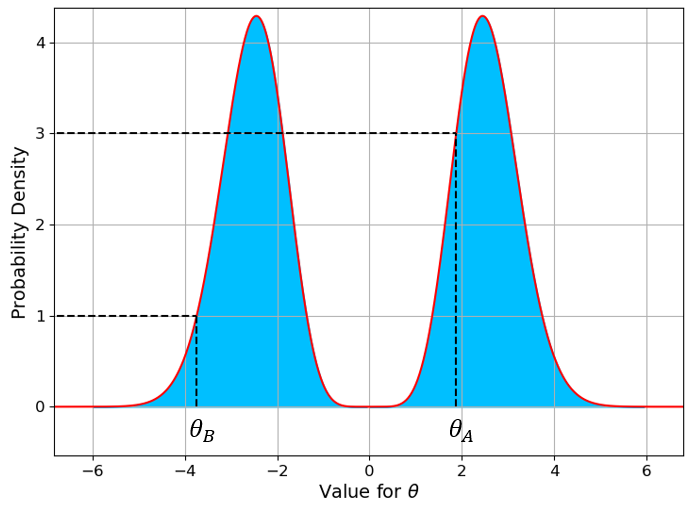
\includegraphics[width = 4.3in]{NormalDistribution.png}
\caption{Plot of the integrand in equation (\ref{1.3}) shown by the red line with the integral being the blue shaded area under graph. It also shows what two values in parameter space would give the frequency $3$ and $1$.}
\label{fig1.1}
\end{figure}
The reason we divide by this integral is to make the blue area under the graph equal to 1. This is what the term normalise refers to. Currently, the area is not equal to one as this is just the plot of what the numerator in Bayes' Theorem would be for this example
\begin{align*}
P(\text{data}\mid\theta)\cdot P(\theta) = \frac{\theta^6}{\sqrt{2\pi}}\cdot\exp\left(-\frac{\theta^2}{2}\right)
\end{align*}
The integral in equation (\ref{1.3}) is difficult to solve analytically so we need another way. Consider 2 points in parameter space and their ratio:
\begin{align*}
\frac{P(\theta_A\mid \text{data})}{P(\theta_B\mid \text{data})} = \frac{3}{1}
\end{align*}
So the sampler would need to generate random samples three times as often from point $\theta_A$ than point $\theta_B$. This is visualised in Figure \ref{fig1.1}. Now we want to use this in practice. But how can we use the relative posterior density to sample from the posterior?

Firstly, let us think more about what the posterior distribution actually is. It is the frequency that we will sample a value for an infinite sample of observations. We can use the relative density of a point versus all others to determine its sampling frequency. To determine the frequency of samples at a given point in parameter space, we do not need the absolute value of the posterior at that point, if we know its value relative to other parameter values.

So, even though we cannot calculate the absolute posterior in general, we can still determine its value. Taking another two points in parameter space, $\theta_C$ and $\theta_D$, we can calculate the ratio of the posterior density at these two parameter values using Bayes' Theorem (equation \ref{1.1})
\begin{align}
\dfrac{P(\theta_C\mid \text{data})}{P(\theta_D\mid \text{data})} &= \dfrac{\dfrac{P(\text{data}\mid\theta_C)\cdot P(\theta_C)}{P(\text{data})}}{\dfrac{P(\text{data}\mid\theta_D)\cdot P(\theta_D)}{P(\text{data})}}\nonumber \\
&= \dfrac{P(\text{data}\mid\theta_C)\cdot P(\theta_C)}{P(\text{data}\mid\theta_D)\cdot P(\theta_D)}\label{1.4}
\end{align}
The tricky denominator term has cancelled out and now everything in equation (\ref{1.4}) is known which gives us the un-normalised posterior. This is enough to give us the sampling frequency at each point in parameter space versus all other points. The reason that the un-normalised posterior tells us everything we need to know about the posterior is because all the shape of the posterior is determined by the numerator of Bayes' Theorem. So now we can write
\begin{align}
P(\theta\mid \text{data}) &= \frac{P(\text{data}\mid \theta)\cdot P(\theta)}{P(\text{data})}\nonumber \\
&\propto P(\text{data}\mid \theta)\cdot P(\theta)\label{1.5}
\end{align}
By only using the likelihood and prior, we can produce an un-normalised posterior which will have all the same properties like the mean and standard deviation. The \bb{mean} is the average of the data and the \bb{standard deviation} is the amount of variation in the data.

(See \cite{3} Chapter 12 for more explanation on dependent sampling)

This chapter has covered all of the important tools that will be used throughout. A quick note that if you are unfamiliar with any of the probability distributions mentioned in this report there are many resources available online where you can learn about each one. Now we are ready to introduce some different sampling algorithms and how they are used in different applications.

\section{Markov Chains}\label{markov chains}
\vspace{-0.4in}
\underline{\hspace{6.2in}}
\vspace{-0.1in}

For completeness, I will define what a Markov chain is as the term state is used in definition \ref{MH def} which relates to this definition. Do not worry if the mathematics is too advanced for you, it is not essential to understand in order to understand the rest of this report.

Markov Chain Monte Carlo (MCMC) is a process for generating samples $x^{(i)}$ while \textit{wondering} the possible states $X = \{x_1,x_2,\ldots,x_n\}$ using the Markov chain mechanism which is constructed so that the samples $x^{(i)}$ replicate samples drawn from the target distribution $P(x)$. A Markov chain on a finite state space where $x^{(i)}$ can take any state $X$ is called a Markov chain if 
\begin{align}\label{Markov Chain Def}
P(x^{(i)}\mid x^{(i-1)},x^{(i-2)},\ldots,x^{(1)}) = P(x^{(i)}\mid x^{(i-1)})
\end{align}

The progression of the Markov chain in a state space $X$ depends only on the current state of the chain and a fixed \textbf{transition} matrix, denoted \textbf{P}. To gather a more intuitive understanding we should see an example.

\subsection{What's for dinner?}\label{What's for Dinner}
\vspace{-0.35in}
\underline{\hspace{6.2in}}
\vspace{-0.1in}

Consider a Markov chain with $3$ states ($n=3$). The corresponding transition matrix, illustrated by Figure \ref{figMarkovProcess}, represents the probabilities of what I am hungry for, given the food I had on the preceding day
\begin{align*}
\textbf{P} = \begin{bmatrix}
	& P & B & H \\
    P & 0.5 & 0.3 & 0.2 \\
    B & 0.25 & 0.5 & 0.25 \\
    H & 0.4 & 0.4 & 0.2
\end{bmatrix}
\end{align*}
This defines the probability of going from a state $x_i$ to $x_j$ where $i,j = 1,2,\ldots,n$. So the element $[\textbf{P}]_{ij}$ is the probability that a day with dinner $i$ will be followed by a day with dinner $j$ e.g. $[\textbf{P}]_{12}$ is a $30\%$ chance that a pizza will be followed by a burger.

\begin{figure}[H]
\centering
\begin{tikzpicture}[auto]
\tikzstyle{node} = [circle, draw,text width=4.5em, text badly centered, node distance=3cm, inner sep=0pt]
\node [node] (node0) {Hotdog};
\node [node,above left of=node0,yshift=1cm] (node1) {Pizza};
\node [node,above right of=node0,yshift=1cm] (node2) {Burger};
\path (node0) edge [bend left,->,thick] node [pos=0.5] { 0.4} (node1);
\path (node1.south east) edge [bend left,->,thick] node [pos=0.5,below left] { 0.2} (node0);
\path (node1) edge [bend left,->,thick] node [pos=0.5] { 0.3} (node2);
\path (node2) edge [bend left,->,thick] node [pos=0.5] { 0.25} (node0);
\path (node2) edge [bend left,->,thick] node [above,pos=0.5] {0.25} (node1);
\path (node2.south west) edge [bend right,<-,thick] node [pos=0.5,below right] {0.4} (node0);
\path (node0) edge [loop below,->,thick] node [pos=0.5] {0.2} (node0);
\path (node1) edge [loop left,->,thick] node [pos=0.5] {0.5} (node1);
\path (node2) edge [loop right,->,thick] node [pos=0.5] {0.5} (node2);
\end{tikzpicture}
\caption{Graph for the transition of state with their corresponding probability.}
\label{figMarkovProcess}
\end{figure}
\newpage
So, say I have pizza for dinner on day $1$. This is represented as the vector
\begin{align*}
{x}^{(1)} = [1,0,0]
\end{align*}

Now the dinner I will have on day $2$ is given by
\begin{align*}
{x}^{(2)} = {x}^{(1)}\textbf{P} = [1,0,0]\begin{bmatrix}
    0.5 & 0.3 & 0.2 \\
    0.25 & 0.5 & 0.25 \\
    0.4 & 0.4 & 0.2
\end{bmatrix} = [0.5,0.3,0.2]
\end{align*}

There is a $50\%$ chance I will have pizza again on day $2$.

The dinner for day $3$ is similar
\begin{align*}
{x}^{(3)} = {x}^{(2)}\textbf{P} = {x}^{(1)}\textbf{P}^2 = [1,0,0]\begin{bmatrix}
    0.405 & 0.38 & 0.215 \\
    0.35 & 0.425 & 0.245 \\
    0.38 & 0.4 & 0.22
\end{bmatrix} = [0.405,0.38,0.215]
\end{align*}

So the general formula for day $n$ is
\begin{align*}
{x}^{(n)} = {x}^{(1)}\textbf{P}^n
\end{align*}

As the days go on, the vector ${x}^{(n)}$ tends to what is called a \textbf{steady state} vector which represents the probability of what I will have for dinner on all days, with the assumption that this is all I will eat for the rest of my days, no matter what the initial meal (distribution) is. This is a very important piece of MCMC simulation. For any initial distribution, the Markov chain will converge to the invariant distribution $P(x)$, represented as
\begin{align}\label{Stationary Vector}
P(x) = P(x)\textbf{P}
\end{align}

Thus,
\begin{align*}
P(x)\textbf{P} = P(x) = P(x)\textbf{I}
\end{align*}
\vspace{-30pt}
\begin{align*}
\Rightarrow\quad P(x)(\textbf{P} - \textbf{I}) &= P(x)\left(\begin{bmatrix}
    0.5 & 0.3 & 0.2 \\
    0.25 & 0.5 & 0.25 \\
    0.4 & 0.4 & 0.2
\end{bmatrix} - \begin{bmatrix}
    1 & 0 & 0 \\
    0 & 1 & 0 \\
    0 & 0 & 1
\end{bmatrix}\right)\\
&= P(x)\begin{bmatrix}
    -0.5 & 0.3 & 0.2 \\
    0.25 & -0.5 & 0.25 \\
    0.4 & 0.4 & -0.8
\end{bmatrix} = \boldsymbol{0}\\
\end{align*}

Note the condition $P_1 + P_2 + P_3 = 1$. Using this we can solve these simultaneous equations to give us the steady state distribution
\begin{align*}
[P_1,P_2,P_3] = [0.3774,0.4025,0.2201]
\end{align*}

This means that, as the days go on, I will have pizza for $37.74\%$, burger for $40.25\%$ and hotdog for $22.01\%$ of days in the future. It is important to note that Equation (\ref{Stationary Vector}) only holds if the transition matrix \textbf{P} satisfies the following conditions:
\begin{itemize}
\item Irreducibility: For any state of the Markov chain, there is a positive probability of visiting
all other states. That is, the matrix T cannot be reduced to separate smaller matrices.
\item Aperiodicity: The chain should not get trapped in cycles.
\end{itemize}

A sufficient, but not necessary, condition to ensure that a particular $P(x)$ is the desired
invariant distribution is the following reversibility condition
\begin{align}\label{reversibility}
P\left(x^{(i)}\right)\textbf{P}\left(x^{(i-1)}\mid x^{(i)}\right) = P\left(x^{(i-1)}\right)\textbf{P}\left(x^{(i)}\mid x^{(i-1)}\right)
\end{align}

Summing both sides over $x^{(i-1)}$ gives
\begin{align*}
P\left(x^{(i)}\right) = \sum_{x^{(i-1)}}P\left(x^{(i-1)}\right)\textbf{P}\left(x^{(i)}\mid x^{(i-1)}\right)
\end{align*}
(See \cite{5} for more detail)

\section{Coding}\label{coding}
\vspace{-0.4in}
\underline{\hspace{6.2in}}
\vspace{-0.1in}

We are going to focus on how these algorithms are used for different problems. All of these methods are numerical approaches so this report will heavily involve numerical implementation which I did in \bb{R} and \bb{Python}. If you have never used (or even heard of) these programming languages that is okay. You will still understand everything from a mathematical perspective. If you are familiar with these languages then you will be able view all of the code that I have written myself through the following link:
\begin{center}
\url{https://github.com/iMikeT/MathProject2}
\end{center}
To run the different Python codes that I have written on your own computer you will need the package Scikit-Learn. And for the R codes I have used the plotting package ggplot2. You will need to install these yourself before running any code. The links to access specific code files for the example I cover will be provided throughout this report.

I have been teaching myself for the last two years how to write in these programming languages, so that I would be able to fully explore the functionality of all the different samplers involved and to move further into the world of machine learning which will come towards the end of this report.

All of the figures presented are my own, generated within the code mentioned above, and links to different animations that I have made will also be available within my GitHub repository link.

I have been able to write all of the Python code for the machine learning processes used in this report through taking free online courses given by edX in collaboration with Microsoft, one of which that was most helpful I will leave a link for you to see \href{https://www.edx.org/course/principles-of-machine-learning-python-edition-2}{here}.

\chapter{Metropolis Algorithms}\label{Metropolis}

These algorithms are the most popular MCMC algorithms for their simplicity. But for some problems these samplers will struggle and we will need something more advanced.

\section{Random Walk Metropolis}\label{Random Walk Metropolis}
\vspace{-0.4in}
\underline{\hspace{6.2in}}
\vspace{-0.1in}

As discussed before, \bb{independent sampling} is generally impossible, and therefore cannot determine exactly the entire structure of the posterior. But we can generate an estimation for it with local exploration using \bb{dependent sampling} i.e. the next sample value will \ti{depend} on the current value. This is easier to implement since it only requires calculation of the un-normalised posterior.

But how do we choose \ti{where} to propose a next step from the current and \ti{whether} we move to it or stay? We need to sample more from the peaks (accept new step) and less from the lower levels (reject or accept) of the posterior probability density function (PDF). This leads us to the definition of the Random Walk Metropolis algorithm.

\vspace{7pt}
\begin{definition}\label{Metropolis Def}
\bb{Metropolis:} Let $f(\theta)$ be a function that is proportional to the posterior distribution $P(\theta\mid \text{data})$ such that
\begin{align*}
P(\theta\mid \text{data}) \propto f(x) = P(\text{data}\mid \theta)\cdot P(\theta)
\end{align*}

where $\theta$ is an $n$-dimensional, continuous parameter, and $n\in\N$ where $\N$ denotes the natural numbers.
\begin{enumerate}
\item Choose an arbitrary point $\theta_0$ for the first sample, and choose a proposal distribution $Q(\theta^\p\mid\theta)$ that suggests a candidate for the next sample value $\theta^\p$, given the previous value $\theta$. For this algorithm, $Q$ must be symmetric which means that \newline$Q(\theta^\p\mid\theta) = Q(\theta\mid\theta^\p)$. A typical choice is the Normal distribution centred at $\theta$.
\item For each iteration $t$ where $t\in\mathbb{Z}$, $t\geq 0:$
\begin{itemize}
\item Generate a candidate $\theta^\p$ for the next sample by sampling from the proposal distribution $Q(\theta^\p\mid \theta_t)$.
\item Calculate the acceptance ratio $r = \dfrac{f(\theta^\p)}{f(\theta_t)}$ where $r$ is the probability that the point in parameter space $\theta^\p$ is accepted as the next sample value. The acceptance ratio will decide to either accept or reject the candidate. Since $f(\theta)$ is proportional to $P(\theta\mid\text{data})$, we have $r = \dfrac{P(\theta^\p\mid\text{data})}{P(\theta_t\mid\text{data})}$ since any constant of proportionality would be cancelled.
\item Accept or reject:
\begin{itemize}
\item Generate a uniform random number $u\in[0,1]$.
\item If $u\leq r$ accept the candidate: $\theta_{t+1} = \theta^\p$.
\item If $u> r$ reject the candidate: $\theta_{t+1} = \theta_t$.
\end{itemize}
\end{itemize}
\end{enumerate}
Here $\mathbb{Z}$ denotes the integers.
\end{definition}

Essentially, we want to take a ``random walk'' through parameter space where the next step is dependent on the current step and the shape of the posterior. The above can be formalised as:
\begin{align}
r=\begin{cases}
	\quad\quad\,\,\,1,&\text{if}\,\,\,P(\theta_{t+1}\mid\text{data})\geq P(\theta_t\mid\text{data})\\
	\dfrac{P(\theta_{t+1}\mid\text{data})}{P(\theta_t\mid\text{data})},&\text{if}\,\,\,P(\theta_{t+1}\mid\text{data})<P(\theta_t\mid\text{data})
\end{cases}\label{2.1}
\end{align}

We can substitute in the un-normalised posterior densities because the denominator cancels out as shown in equation (\ref{1.4}). To visualise this process more clearly, we can consider an example.

\subsection{A Stroll Through a Strange Park}\label{Metropolis Example}
\vspace{-0.35in}
\underline{\hspace{6.2in}}
\vspace{-0.1in}

Suppose we have a posterior density function that is not normalised. This means that we have the following:
\begin{align*}
P(x\mid \text{data}) = P(\text{data}\mid x)\cdot P(x)
\end{align*}

taking $x$ as the parameter variable instead of $\theta$. Figure \ref{fig1.2} shows a plot of the following equation:
\begin{align*}
P(\text{data}\mid x)\cdot P(x) = \frac{\exp\bkt{-\dfrac{(x - 0.2)^2}{0.002}}}{\sqrt{\dfrac{6}{5}\pi}} + \frac{\exp\bkt{-\dfrac{(x - 0.45)^2}{0.02}}}{\sqrt{\dfrac{2}{5}\pi}} + \frac{\exp\bkt{-\dfrac{(x - 0.7)^2}{0.002}}}{\sqrt{\dfrac{4}{5}\pi}}
\end{align*}

So the posterior PDF is a combination of three normal distributions. In this example, we are going to sample from this function using the Random Walk Metropolis algorithm defined in definition \ref{Metropolis Def}. Lets run the sampler for 200 iterations and see what happens.
\begin{figure}[H]
\centering
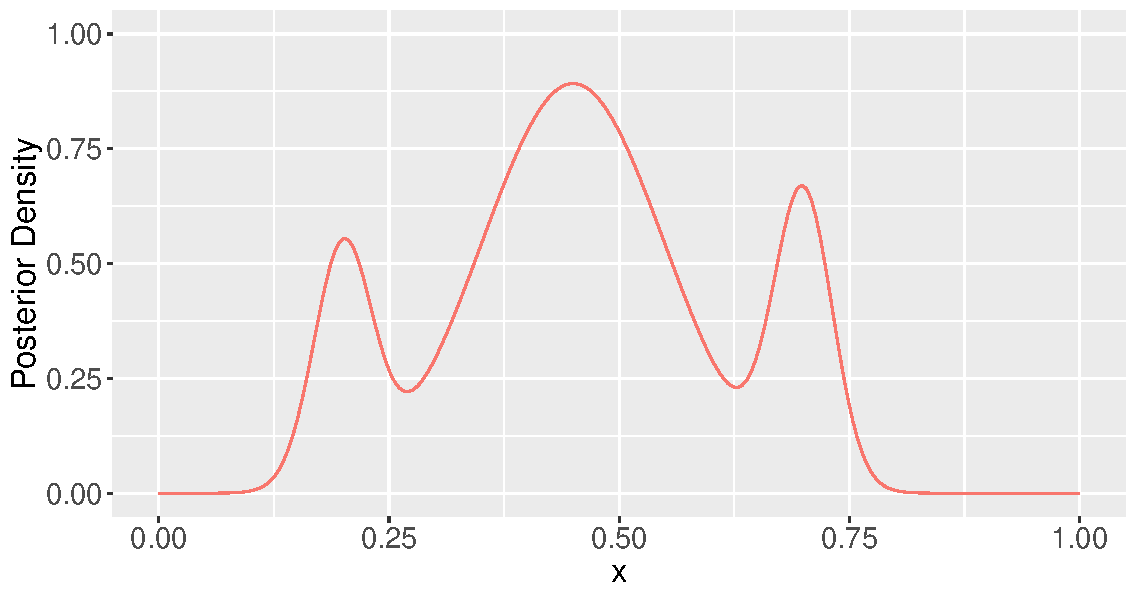
\includegraphics[width = 4.3in]{exact.pdf}
\vspace{-12pt}
\caption{Plot of the exact posterior we want the sampler to estimate. We will use this to comment on the accuracy of the Random Walk Metropolis algorithm.}
\label{fig1.2}
\end{figure}

\begin{figure}[H]
\centering
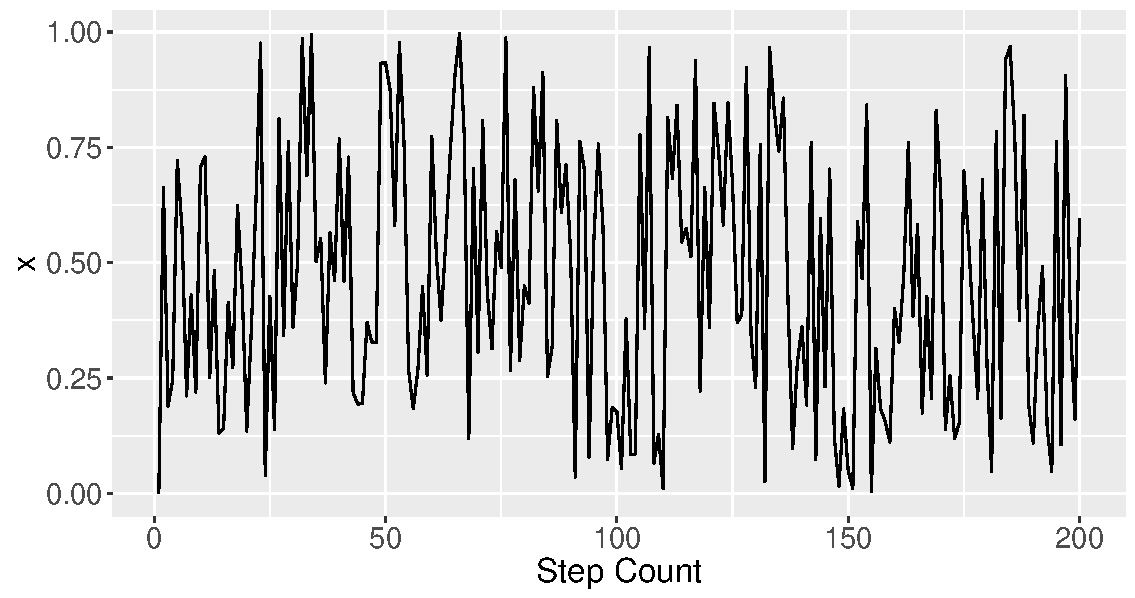
\includegraphics[width = 4.3in]{200wiggly.pdf}
\caption{Plot of how the parameter $x$ randomly ``walks'' through parameter space in each iteration of the algorithm.}
\label{fig1.3}
\end{figure}

Figure \ref{fig1.3} shows how the algorithm moves through different values for the parameter $x$ by accepting the proposed values over 200 iterations. Because each $(n+1)$-th value depended on the $n$-th value we can track the accepted step $(n+1)$ and link it to the previous step $n$ with a straight line to visualise how each accepted proposed candidate is dependent from the previous value. This produces an entire web presented in Figure \ref{fig1.4}.
\begin{figure}[H]
\centering
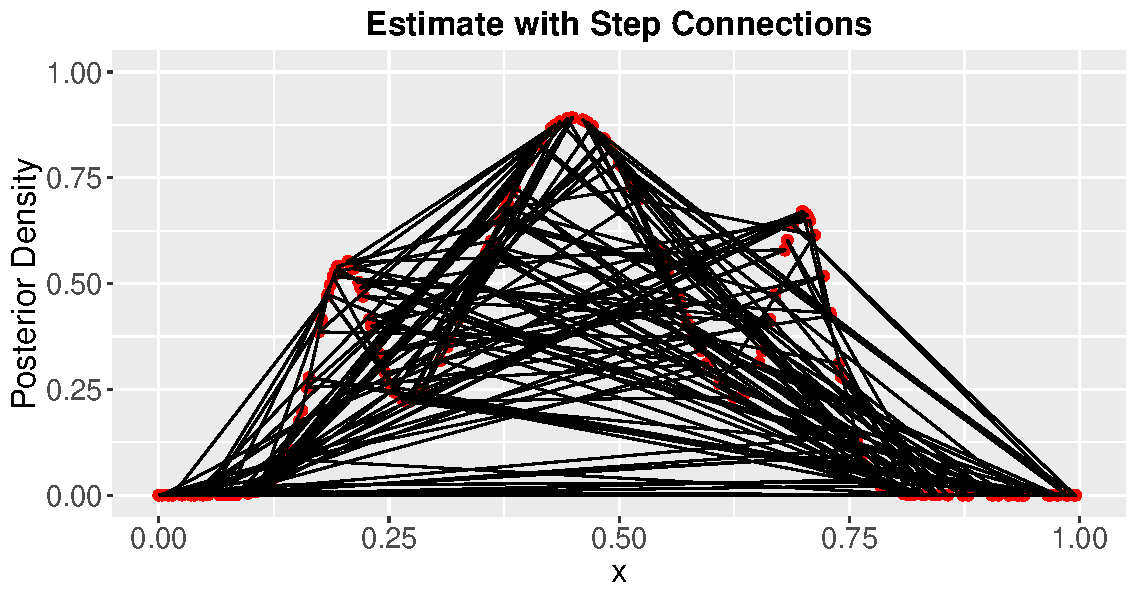
\includegraphics[width = 4.3in]{200approx.pdf}
\caption{Plot of how each point of the posterior estimate is connected to the previous point.}
\label{fig1.4}
\end{figure}

We can then strip away the connections and plot a line through each of the points to determine the accuracy of the sampler given in Figure \ref{fig1.5}.
\begin{figure}[H]
\centering
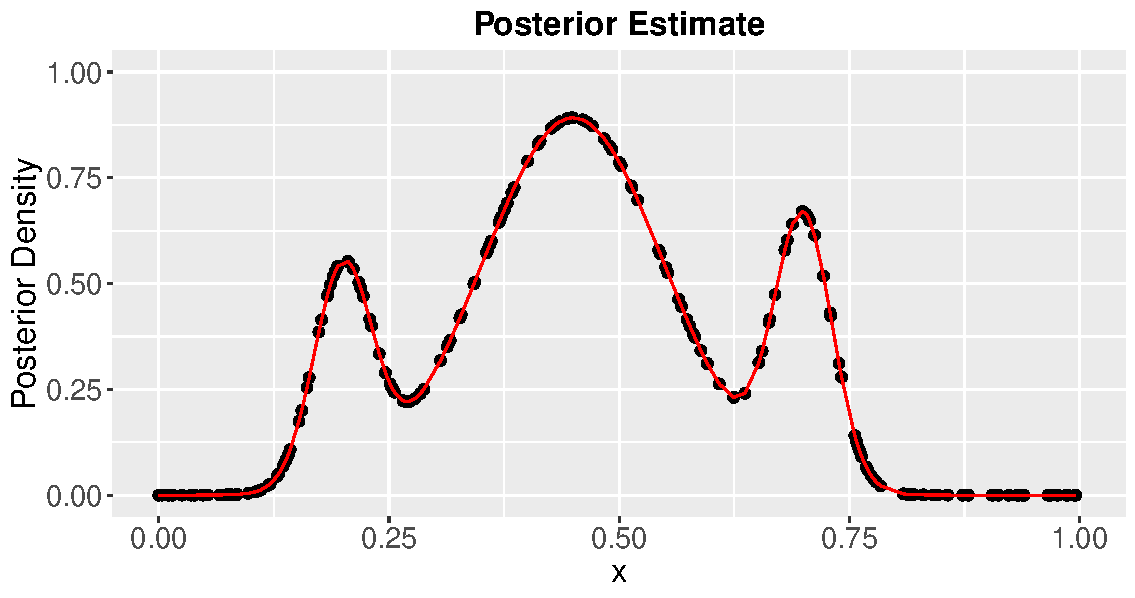
\includegraphics[width = 4.3in]{200point.pdf}
\caption{Plot of the posterior approximation after 200 iterations without connections.}
\label{fig1.5}
\end{figure}

The estimation is very accurate to the exact graph. In a more real world application, we will not have the posterior as an exact graph. We will want to produce a posterior distribution for the parameter(s) that will then be used to generate a model from some data. 

Using a continuous graph helps illustrate more clearly how the algorithm moves. We can now try applying a similar MCMC sampler to some data in another example.

(For the code used in this example visit this \href{https://github.com/iMikeT/MathProject2/tree/master/R%20Code/Metropolis/Metropolis%20Example}{link}.)
\pagebreak
\section{Metropolis Hastings}\label{Metropolis Hastings}
\vspace{-0.4in}
\underline{\hspace{6.2in}}
\vspace{-0.1in}

Lets take a brief moment to discuss the difference between Metropolis-Hastings and Metropolis sampling algorithms. It was mentioned in definition \ref{Metropolis Def} that the Metropolis algorithm must have a symmetric proposal distribution. If there are boundary conditions in parameter values, say at zero, then a symmetric distribution can produce a negative value for the standard deviation $\sigma$. So, if we then reject all steps where $\sigma < 0$, we will generate few samples from parameter space where $\sigma$ is close to zero.

Thinking about this more, the areas near zero are only able to be reached by the positive side of $\sigma$. This is very different from higher parameter values which can be reached by both sides of $\sigma$, meaning that we produce too few samples near zero. So the Metropolis algorithm does not work when there are boundaries in parameter values, like we will have in next example.

Taking a look at Figure \ref{fig1.7} shows what we mean by this negative $\sigma$. Say we have accepted a sample at parameter value 0.04, then we would take this value as the mean of a normal proposal distribution and generate a new sample candidate. The problem comes here when we have a boundary constraint at zero. All the values that would be given in the shaded region would be rejected and we would keep stepping back to 0.04 until we generate a candidate in the positive parameter space. This is what causes asymmetry in the sampler which Metropolis cannot handle.
\begin{figure}[H]
\centering
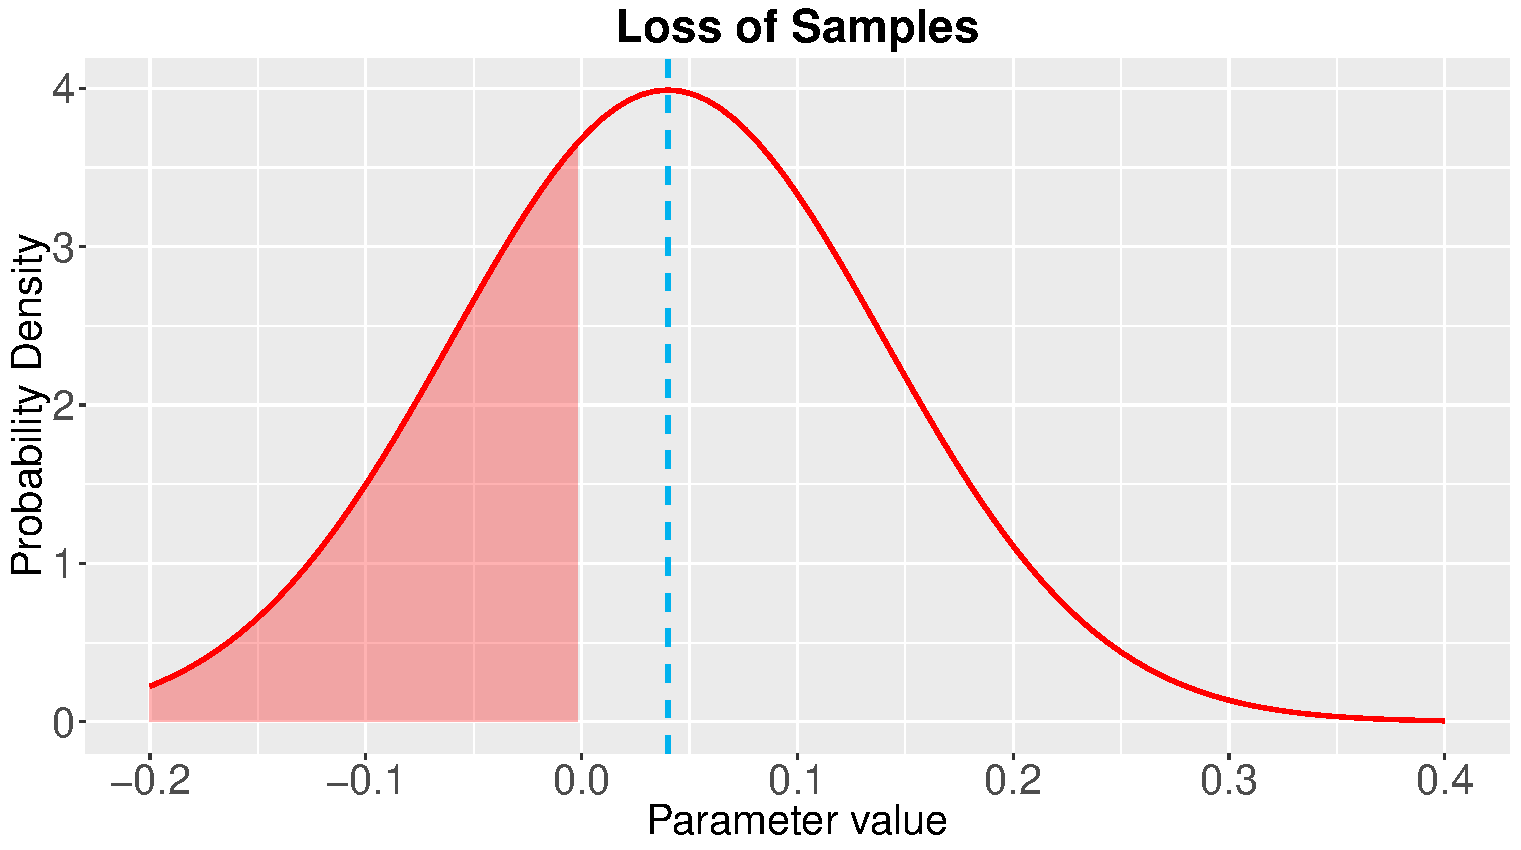
\includegraphics[width = 4.3in]{Lostsamples.pdf}
\caption{Plot of a symmetric proposal distribution, shown using a red line, with a shaded region that shows all of the potential samples we would lose due to a boundary constraint at zero. The blue dashed line is the mean of the proposal distribution; which would be the current parameter value in the sampling algorithm.}
\label{fig1.7}
\end{figure}

So we need to change the sampler and it turns out that we have been using a special case of another sampler. The Metropolis-Hastings algorithm is a modified Metropolis algorithm that allows an asymmetric proposal distribution. And that when we choose a symmetric proposal distribution, it resorts back to the Metropolis algorithm.

An asymmetric proposal distribution will always produce parameter values within the boundary of parameter space i.e. only positive values. Lets see how this algorithm is different.

\vspace{7pt}
\begin{definition}\label{MH def}
\bb{Metropolis-Hastings:}
\begin{enumerate}
\item Pick a random initial state $x_0$.
\item For each iteration $t$:
\begin{itemize}
\item Randomly generate a candidate state $x^\p$ from proposal distribution $Q(x^\p\mid x_t)$.
\item Calculate the acceptance ratio
\begin{align*}
A(x^\p,x_t) = \min\left\{1,\dfrac{\big(p(\text{data}\mid x^\p)\cdot p(x^\p)\big)}{\big(p(\text{data}\mid x_t)\cdot p(x_t)\big)}\cdot\dfrac{Q(x_t\mid x^\p)}{Q(x^\p\mid x_t)}\right\}
\end{align*}
\item Accept of reject:
\begin{itemize}
\item Generate a uniform random number $u\in[0,1]$.
\item If $u\leq A(x^\p,x_t)$, accept the new state: $x_{t+1} = x^\p$.
\item If $u>A(x^\p,x_t)$, reject the new state: $x_{t+1} = x_t$.
\end{itemize}
\end{itemize}
\end{enumerate}
\end{definition}
Notice how the first part of acceptance ratio is the same as the Metropolis and the second is the correction for the asymmetric stepping. When the proposal distribution is symmetric we have $Q(x_t\mid x^\p) = Q(x^\p\mid x_t)$ which would then cancel out the right term leaving us with the special case of the Metropolis-Hastings algorithm known as just Metropolis. Now we can be sure that no asymmetries will prevent convergence to the un-normalised posterior.

\subsection{The Lifespan of a Monster}\label{Metropolis-Hastings Example}
\vspace{-0.35in}
\underline{\hspace{6.2in}}
\vspace{-0.1in}

Suppose that we wanted to research the behaviour of malaria carrying mosquitoes. The most important factor is to estimate the lifespan of a mosquito since the longer it lives, the greater chance it has of becoming infected through biting a human with malaria; surviving the period where the malaria parasite migrates to the salivary glands; and passing the disease on through biting an uninfected human.

One method we can use to collect data is to release 1000 young mosquitoes where each one has been marked. On each day $t$ we use a large number of traps to capture mosquitoes and count the number of marked mosquitoes $X_t$. We then release all mosquitoes and repeat the process for 15 days in total.

Since $X_t$ is a count variable and we assume that the recapture of an individual marked mosquito is independent and identically distributed, we can choose a Poisson model
\begin{align}
X_t\sim\text{Poisson}(\lambda_t),\quad\lambda_t = 1000e^{-\mu t}\psi\label{2.2}
\end{align}

Here $\lambda_t$ is the mean, $\mu$ is the mortality rate (assume constant), and $\psi$ is the daily recapture probability. We can use a prior Gamma distribution $\Gamma(2,20)$ for $\mu$ and a prior Beta distribution Beta$(2,40)$ for $\psi$. For a Gamma distribution the mean is $2/20 = 0.1$, and for the Beta distribution the mean is $2/(2+40)\approx0.05$. Substituting this into the equation for $\lambda_t$ and plotting the result along time $t$ we have the following figure.
\begin{figure}[H]
\centering
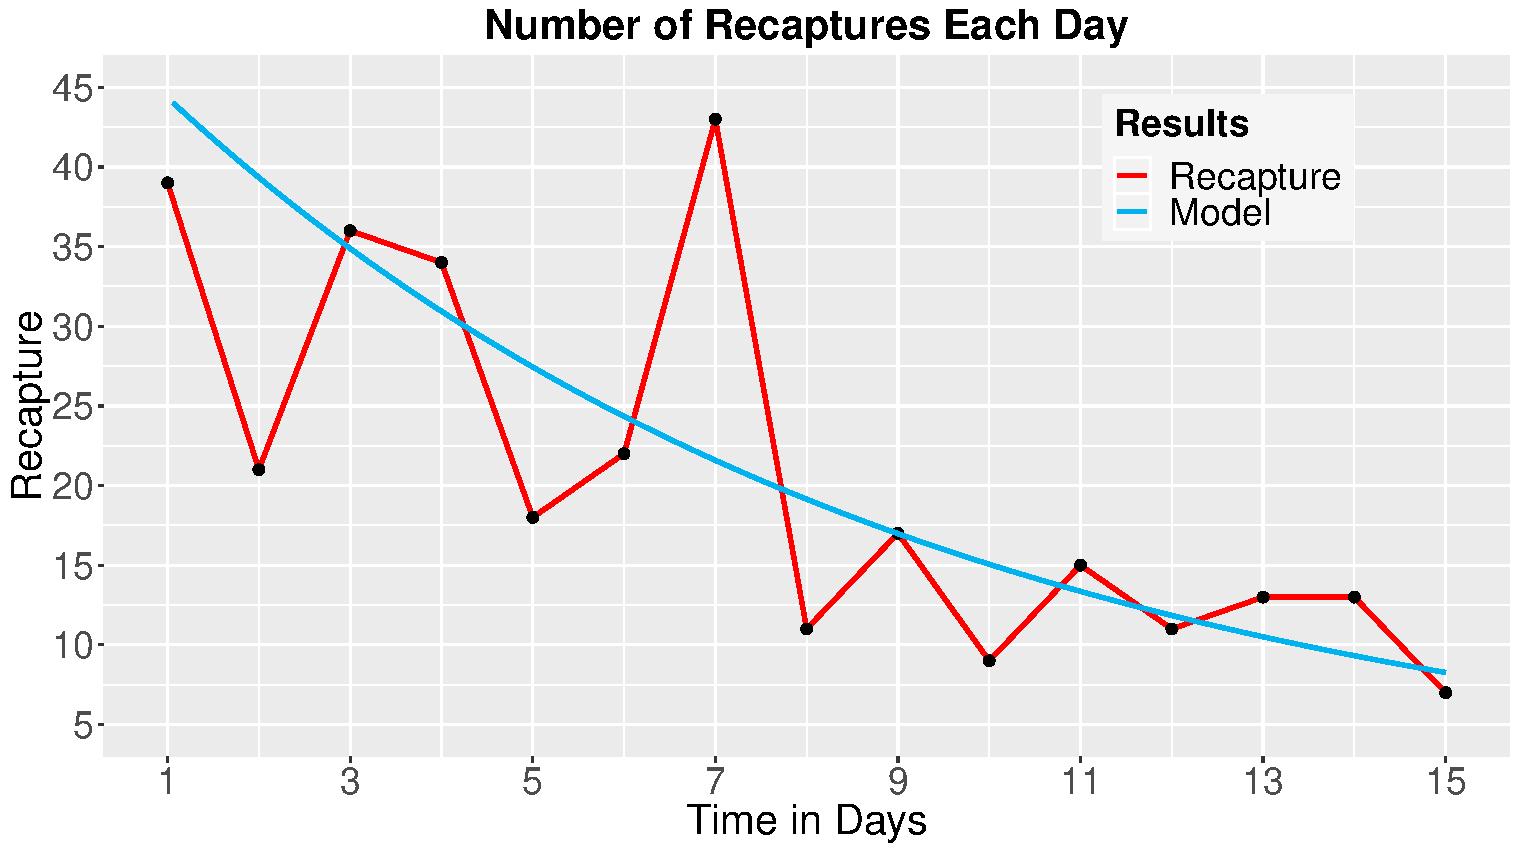
\includegraphics[width = 4.3in]{Recapture.pdf}
\caption{Plot of the recapture data using a red line and the Poisson model with mean $\lambda_t = 1000\times\exp(-0.1\times t)\times0.05$ using a blue line.}
\label{fig1.6}
\end{figure}

We have two prior distributions for the two parameters and a likelihood of the Poisson distribution. Then taking the product of these will give us the numerator of Bayes' Theorem which we know is proportional to the posterior.

We still need to propose a proposal distribution so we can calculate the acceptance ratio. We can use a log-Normal proposal with mean at the current $\mu$ value, and a Beta$(2+\psi,40+\psi)$ proposal for $\psi$. These distributions are asymmetric and so will always be positive, making sure we have no boundary issues.

Now we are ready to substitute this into the Metropolis-Hastings algorithm and record the result. Figure \ref{fig1.8} is a collection of graphs showing different information we can extract from the algorithm.
\begin{figure}[H] 
  \begin{subfigure}[b]{0.5\linewidth}
    \centering
    \hspace{-13pt}
    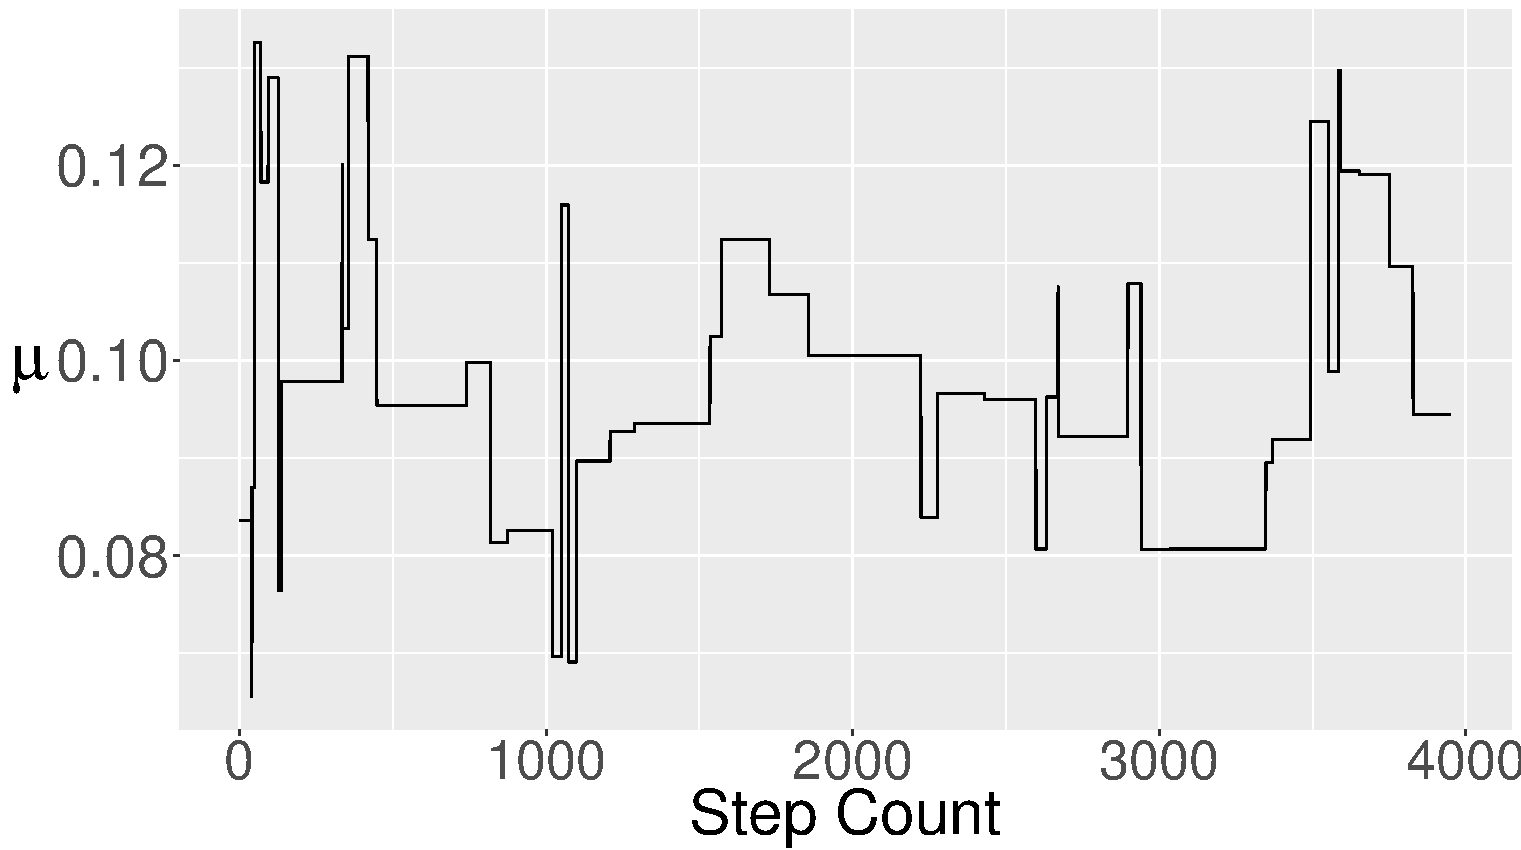
\includegraphics[width=3in]{muwiggly2.pdf}
    \label{fig1.8:a}
  \end{subfigure}
  \begin{subfigure}[b]{0.5\linewidth}
    \centering
    \hspace{-13pt}
    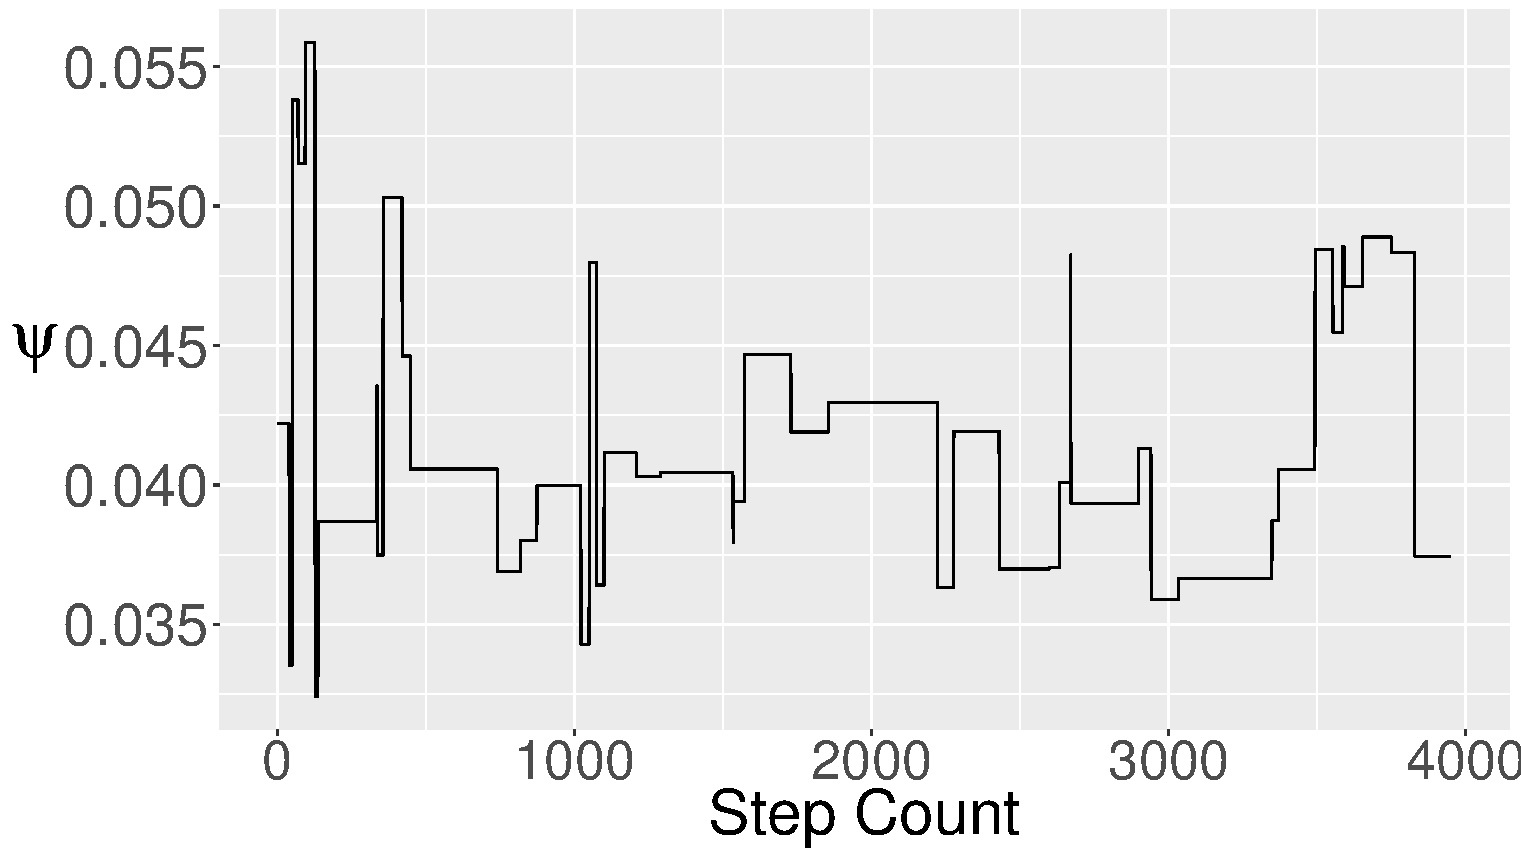
\includegraphics[width=3in]{phiwiggly2.pdf}
    \label{fig1.8:b}
  \end{subfigure}\hfill%
  \begin{subfigure}[b]{0.5\linewidth}
    \centering
    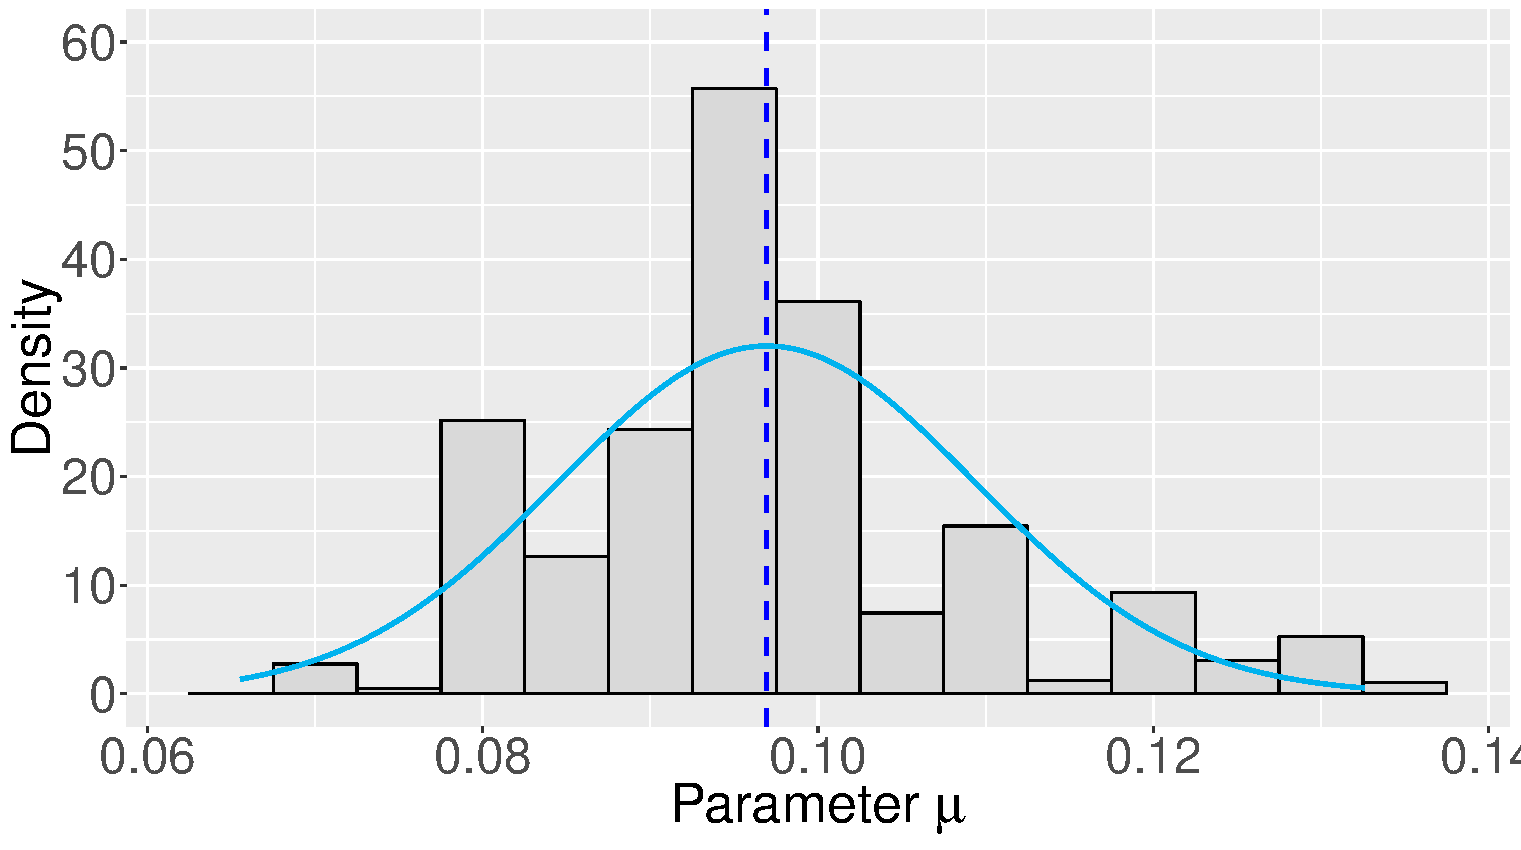
\includegraphics[width=2.9in]{muhist2.pdf} 
    \label{fig1.8:c} 
  \end{subfigure}
  \begin{subfigure}[b]{0.5\linewidth}
    \centering
    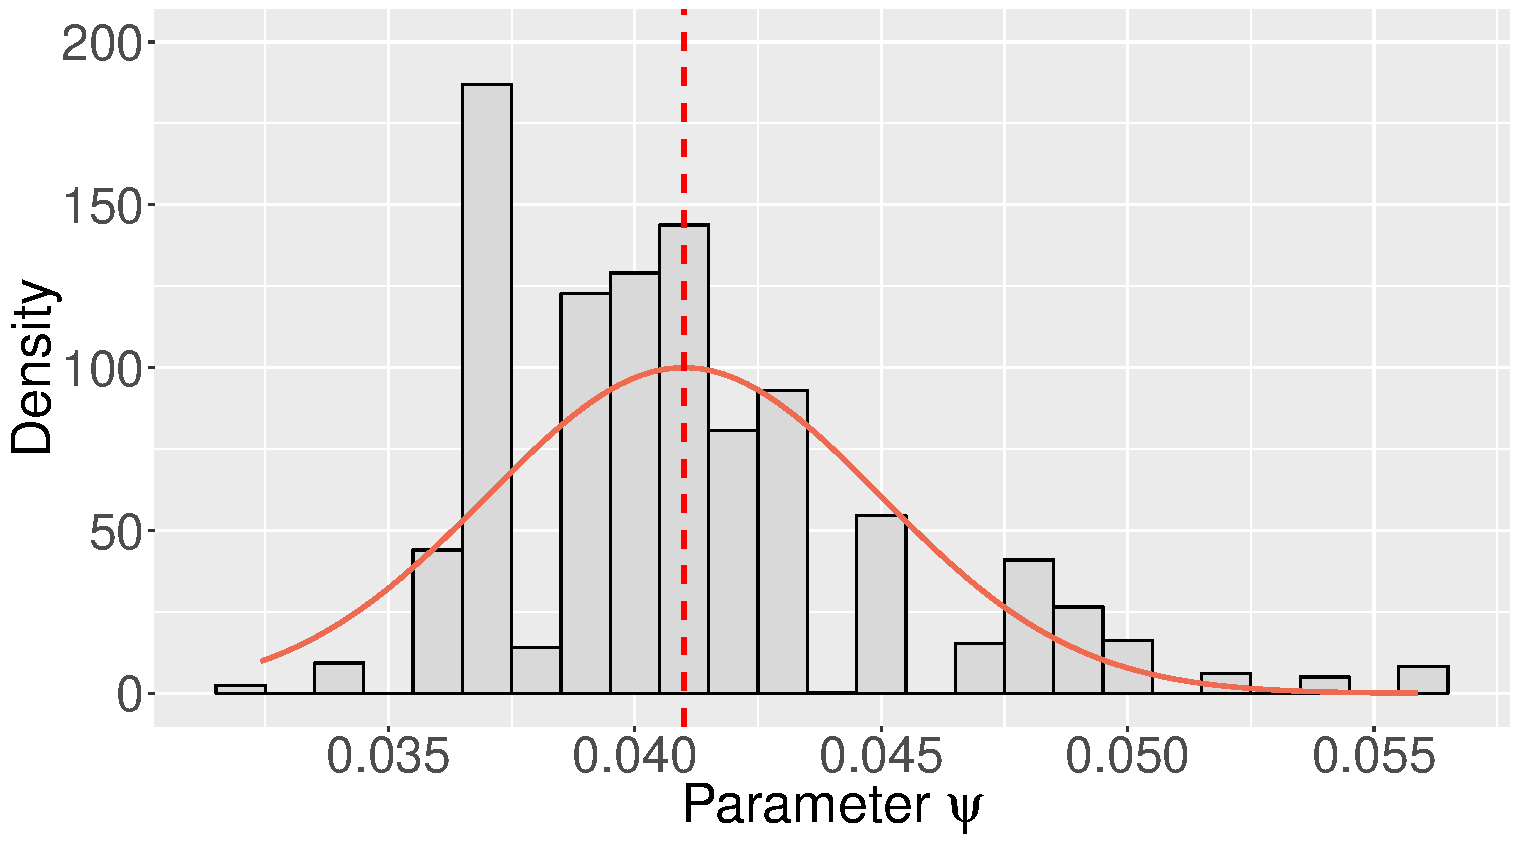
\includegraphics[width=2.9in]{phihist2.pdf}
    \label{fig1.8:d} 
  \end{subfigure} 
  \caption{The two graphs at the top show the values that parameters $\mu$ and $\psi$ take with each iteration. The ``flat'' sections are for when many potential samples were rejected and the algorithm returned to the previous sample. The bottom graphs show the histogram along with the probability density function and the mean value for parameters $\mu$ and $\psi$. PDFs are plotted using solid lines and means are plotted using dashed lines.}
  \label{fig1.8} 
\end{figure}

These two histograms represent the estimated posterior distributions for the two parameters. This is the finished product of the Metropolis-Hastings algorithm but we can take it one step further and show what these posterior distributions \ti{really} represent in this real world problem. After running the sampler with 4000 iteration and removing the first 50 values, as these are the values used to converge, we have the parameter mean estimates
\begin{align*}
\mu &= 0.096937 \pm \sigma_\mu,\quad\sigma_\mu = 0.012458\\
\psi &= 0.040997 \pm \sigma_\psi,\quad\sigma_\psi = 0.003988
\end{align*}
where $\sigma_{\mu,\psi}$ is the standard deviation for each parameter. So the algorithm has generated two posterior distributions, each with their own mean and standard deviation which can be through of as a \bb{confidence interval}. Plus and minus one standard deviation is equivalent to saying that I am 68.2\% confident that the parameter values lie within the intervals
\begin{align*}
0.084479 \leq &\mu \leq 0.109395\\
0.037009 \leq &\psi \leq 0.044985
\end{align*}
The idea of confidence intervals is shown in the Figure \ref{fig1.9}. Here we see how the two parameters are constrained i.e as $\mu$ increases so too does $\psi$. We plot these constraints using all of the accepted parameter values from the 4000 iterations.
\begin{figure}[H]
\centering
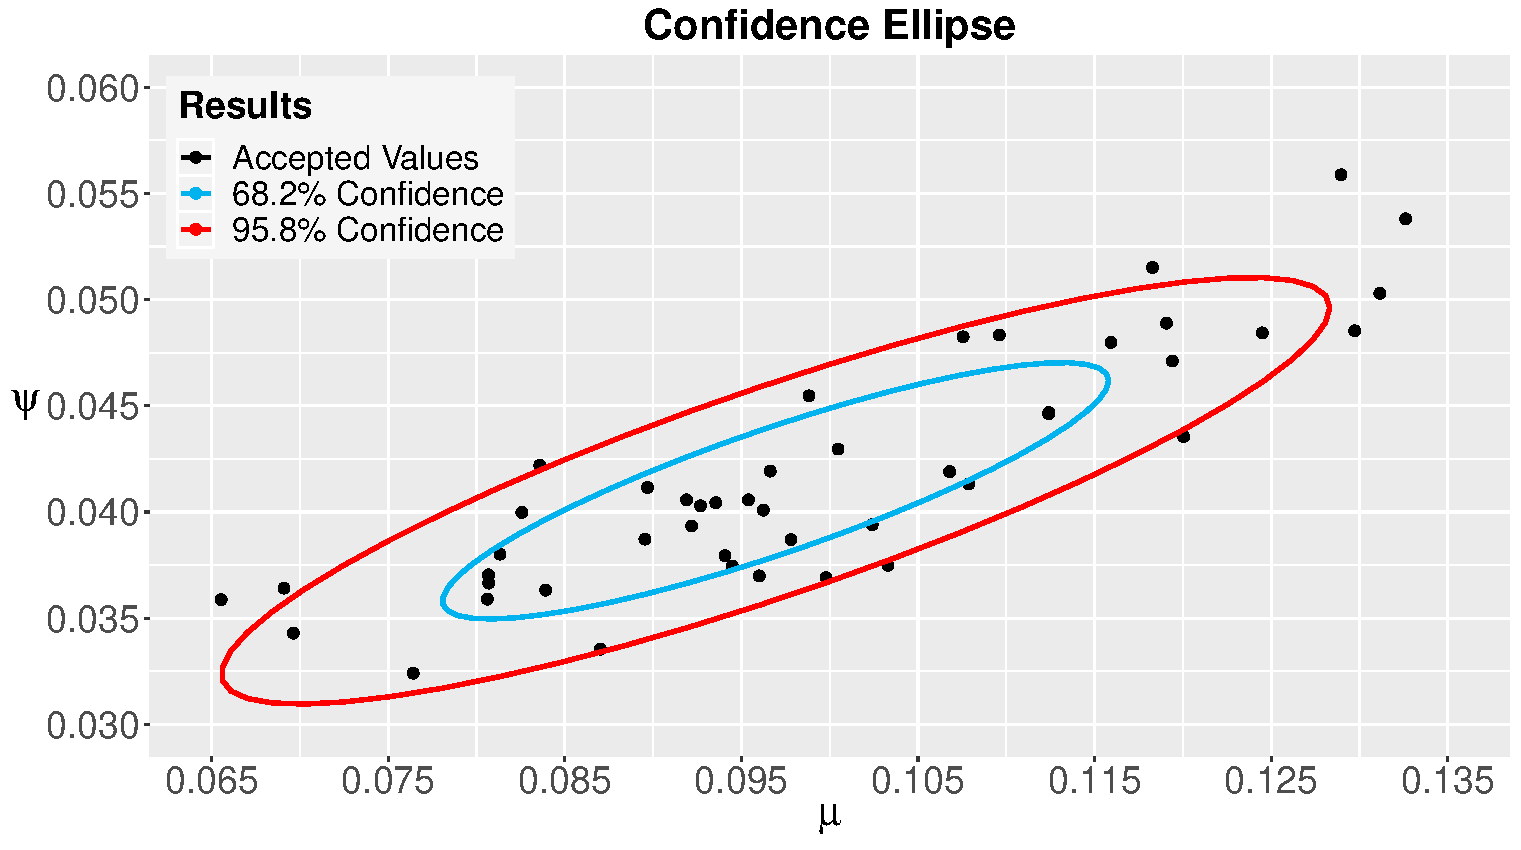
\includegraphics[width = 4.3in]{ellipse2.pdf}
\caption{Plot of the confidence ellipse for 68.2\% which is equal to 1 standard deviation in blue and 95.8\% which is equal to 2 standard deviations in red.}
\label{fig1.9}
\end{figure}

This might not look like much but this is the problem finished! We have used only the data along with different prior, likelihood and proposal distributions to produce an estimated value for the mortality rate $\mu$ and the daily recapture probability $\psi$. Now we can uses all of these accepted samples to plot the original Poisson model along with the original data shown in Figure \ref{fig1.10}.
\begin{figure}[H]
\centering
\includegraphics[width = 4.3in]{Finalmosquito.pdf}
\caption{Final plot of the model for estimating mosquito lifetime using the accepted values shown in Figure \ref{fig1.9}. The best fit line is plotted with the mean values of $\mu$ and $\psi$ using a blue line. The shaded region shows the confidence intervals. The darker region is a 68.2\% confidence interval ($1\sigma_{\mu,\psi}$) and the lighter region is a 95.8\% confidence interval ($2\sigma_{\mu,\psi}$)}
\label{fig1.10}
\end{figure}

(For the code used in this example visit this \href{https://github.com/iMikeT/MathProject2/tree/master/R%20Code/Metropolis/Metropolis-Hastings%20Example}{link}.)

(See \cite{3} Chapter 13 for more detail on \S\ref{Random Walk Metropolis} and \S\ref{Metropolis Hastings})
\chapter{Gibbs \& Bayesian Networks}\label{Gibbs}

After all of that you might be thinking ``this is great!'' and you would not be wrong, but is there something better? The main goal for these algorithms is not just to predict a posterior, but how fast they \ti{converge} to the posterior as well. Here we found a good estimate for the parameters but after 4000 iterations which could be quite demanding for weaker hardware. For this reason I will introduce another MCMC sampling algorithm that has the potential to converge much faster, but it too comes with it own disadvantages.

The Metropolis algorithms are great MCMC samplers because of their simplicity but there is the requirement to fine tune the proposal distribution for each new model. They are also \bb{rejection} algorithm which means we lose many potential steps and limits the algorithms ability to explore parameter space quickly.

This is where Gibbs sampler is different. It accepts every proposal step in parameter space. But how is this possible without being able to independently sample from the posterior distribution? The trick is that we can calculate the \bb{conditional} distribution of the parameters meaning that, if we can independently sample from these conditional distributions, then we can accept all proposed steps, thus increasing the rate of convergence.

Though it may not be possible in most cases to find, and independently sample from,  the conditional distributions for all parameters, we should be able to for some. We would then use Gibbs sampler for these parameters and a Metropolis-like algorithm for the remaining parameters.

\section{The Gibbs Sampler}\label{The Gibbs Sampler}
\vspace{-0.4in}
\underline{\hspace{6.2in}}
\vspace{-0.1in}

It may seem like Gibbs is better than Metropolis in every way so we should list the potential problems. Firstly, we must be able to calculate conditional distributions which might not be possible at all. Secondly, Gibbs can, in fact, be slow to explore parameter space when there is a strong correlation between parameters.

The previous samplers have functioned by proposing a new point and moving there if the posterior probability is greater than the previous point, or based on a probability which depends on the ratio of the new and old points posterior probabilities. Figure \ref{fig3.1} shows how the Metropolis sampler moves through parameter space for both parameters. The Gibbs sampler behaves very differently which we will see in the next example. For now, we'll explore how the Gibbs algorithm works.
\begin{figure}[H]
\centering
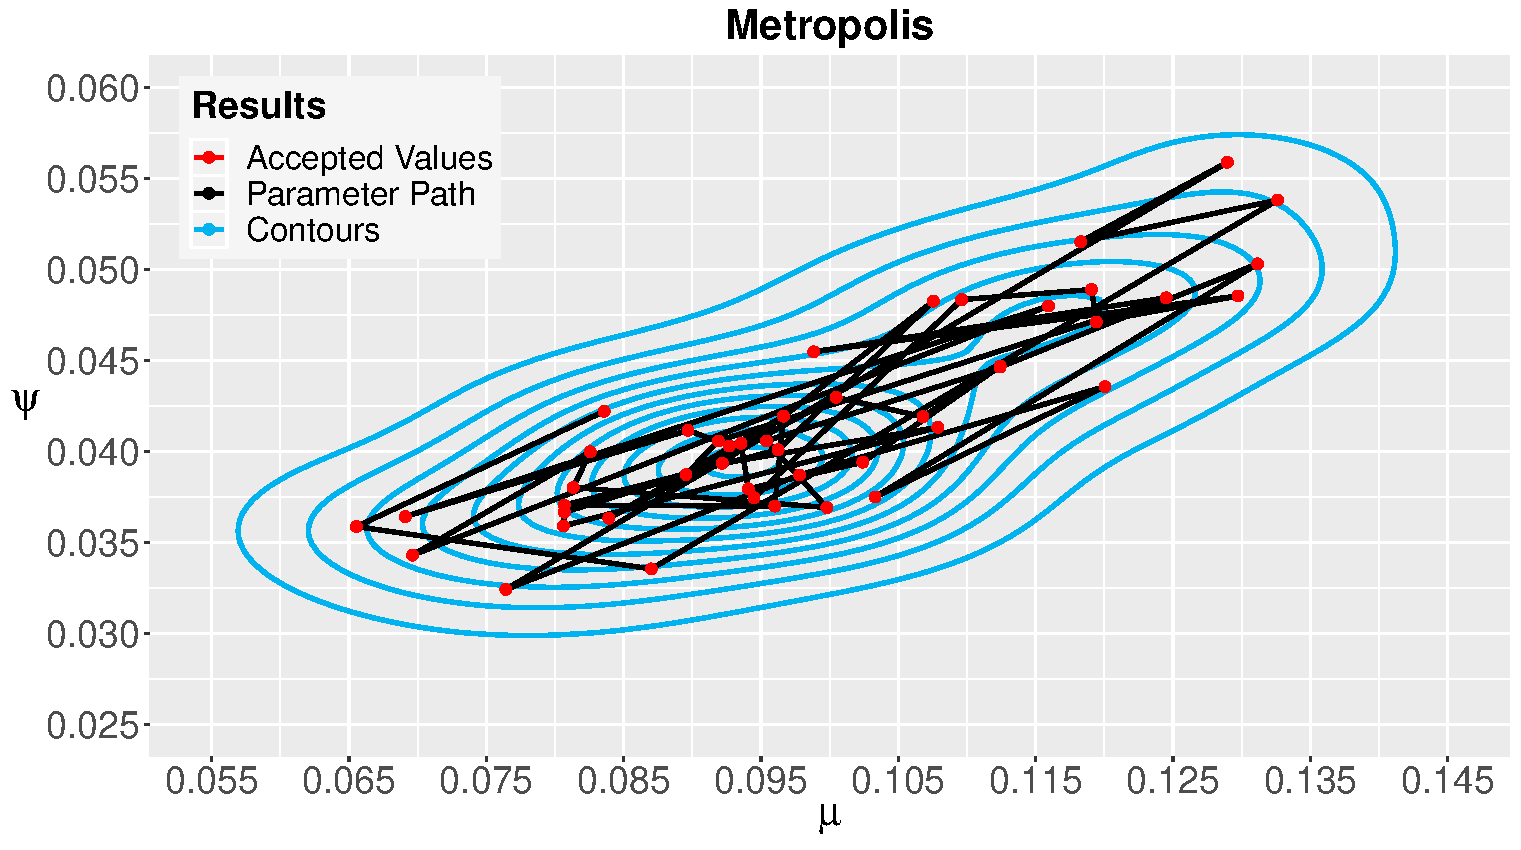
\includegraphics[width = 4.3in]{Metropolispath.pdf}
\caption{This graph shows the path between all of the accepted parameter values for the Metropolis-Hastings algorithm. Notice how, after 4000 iteration, only 46 values were accepted. Though here we have converged to a good estimate in this run, it shows how the high rate of rejection can impede the algorithms ability to converge. Many more iterations are required to increase the reliability of the algorithm.}
\label{fig3.1}
\end{figure}

An important note before we begin is that Gibbs sampling is only \ti{valid} for models with two or more parameters. So to define Gibbs we will use three.
\vspace{7pt}
\begin{definition}\label{gibbs def}
\bb{Gibbs:} Say we have a model with three parameters $\bm{\theta} = (\theta_1, \theta_2, \theta_3)$ and data sample $\bm{\gamma}$. Assume that we can analytically calculate the three conditional distributions given by:
\begin{align*}
P(\theta_1\mid\theta_2, \theta_3,\bm{\gamma}),\quad P(\theta_2\mid\theta_1, \theta_3,\bm{\gamma}),\quad P(\theta_3\mid\theta_1, \theta_2,\bm{\gamma})
\end{align*}
Now we do the following
\begin{enumerate}
\item Choose a random starting point $(\theta_1^0, \theta_2^0, \theta_3^0)$.
\item Choose a random parameter update ordering, say $(\theta_3, \theta_2, \theta_1)$.
\item Sample from the conditional distribution for each parameter using the most recent parameter value. So, for $(\theta_3, \theta_2, \theta_1)$, we would independently sample from
\begin{align*}
P(\theta_3^1\mid\theta_1^0, \theta_2^0,\bm{\gamma})\rightarrow P(\theta_2^1\mid\theta_1^0, \theta_3^1,\bm{\gamma})\rightarrow P(\theta_1^1\mid\theta_2^1, \theta_3^1,\bm{\gamma})
\end{align*}
This is repeated until the sampler has converged.
\end{enumerate}
\end{definition}

Since the Gibbs sampler functions on conditional distributions, it works well when paired with models known as \bb{Bayesian networks}. These are a probabilistic graphical model that uses Bayesian inference for computations. They model joint probability distributions through conditional independence. Before we begin with Bayesian networks consider the following example.

\subsection{Crime \& Unemployment}\label{Crime Example}
\vspace{-0.35in}
\underline{\hspace{6.2in}}
\vspace{-0.1in}

Say that the posterior distribution for the unemployment $u$ and crime levels $c$ for a city is estimated to be a bivariate normal distribution which is a normal distribution generalised to two dimensions. Because we can sample independently from the bivariate normal distribution we don't actually need to perform MCMC on this problem but it will be very useful to show in more detail the movement of Gibbs sampler. 

For a bivariate normal distribution, the conditional distributions are simple and have the nature of a normal distribution. So, performing a similar process as in definition \ref{gibbs def}, we will first choose a random initial state for $u^0$ and $c^0$. Then randomly choose which state to update, say $u^0$. And finally, sample from the conditional distributions with $u^1\mid c^0$. If the next iteration chose to update $c^0$ then we would sample from the conditional density $c^1\mid u^1$. Repeating this process multiple times gives us the following figure.
\begin{figure}[H]
\centering
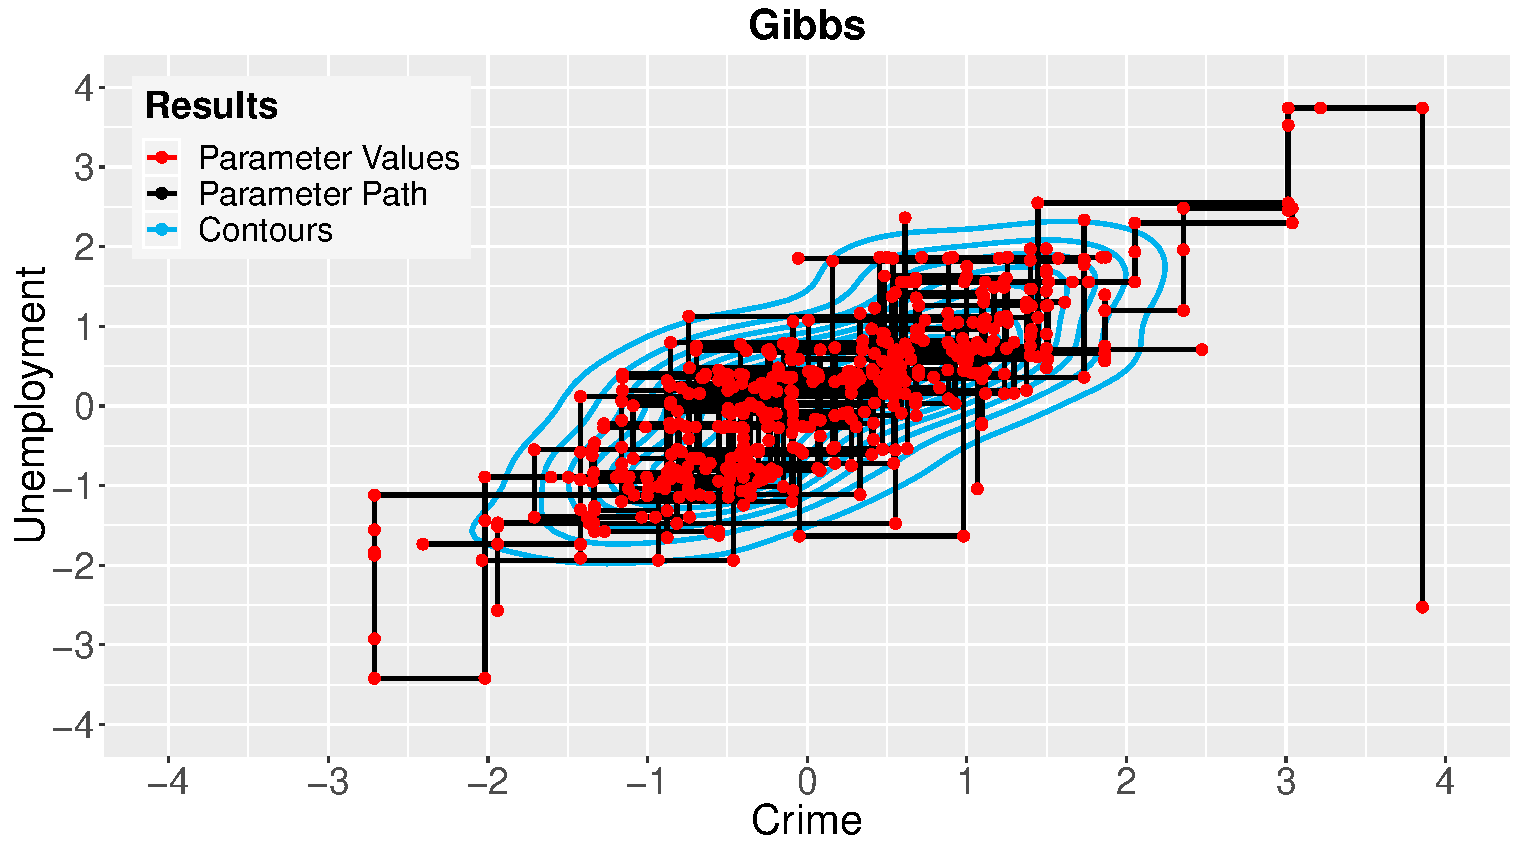
\includegraphics[width = 4.3in]{Gibbspath.pdf}
\caption{This graph shows the path for all parameter values of the Gibbs algorithm. Here there is no reject or accept condition like the Metropolis algorithm. All the parameter values are accepted allowing for faster convergence. This was produced using 500 iterations, far less than the Metropolis algorithms would need to converge.}
\label{fig3.5}
\end{figure}
If you look back at Figure \ref{fig3.1} you see how the nature of the Metropolis-Hastings algorithm is different to the Gibbs algorithm. Because Gibbs chooses to update one parameter with each iteration this produces a rectangular relation between the points. But, when there is a very strong correlation between the two distributions, Gibbs sampler can struggle to explore parameter space and we might need to resort back to the Metropolis algorithm. It goes to show that only using one algorithm for every problem is not wise. Understanding the features of the problem can aid us to choose the sampling algorithm best suited for those features.
\begin{figure}[H]
\centering
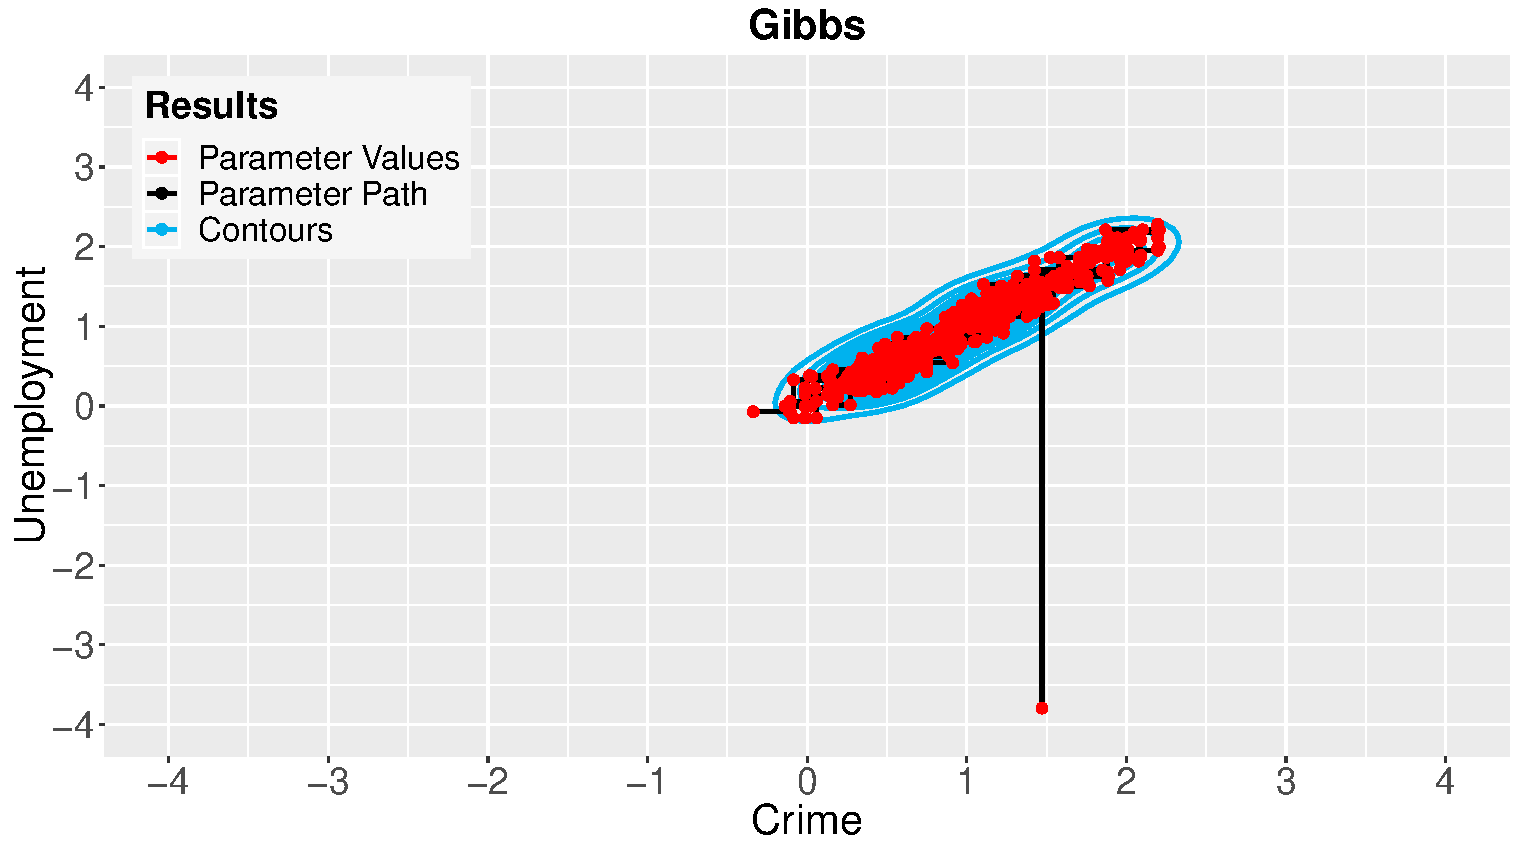
\includegraphics[width = 4.3in]{Gibbsbad.pdf}
\caption{This graph shows how the Gibbs algorithm struggles to explore parameter space when there is a strong correlation between the parameter.}
\label{fig3.6}
\end{figure}
(For the code used in this example visit this \href{https://github.com/iMikeT/MathProject2/tree/master/R%20Code/Gibbs/Crime%20%26%20Unemployment%20Example}{link}.)

Now that we have a good understanding for how the Gibbs sampler is different from the Metropolis samplers we can try an in depth example using Bayesian networks mentioned after definition \ref{gibbs def}. Consider the following figure

\begin{figure}[H]
\centering
\begin{tikzpicture}[
  node distance=1cm and 0cm,
  mynode/.style={draw,ellipse,text width=1.5cm,align=center}
]
\node[mynode] (cl) {Cloudy};
\node[mynode,below left=of cl] (sp) {Sprinkler};
\node[mynode,below right=of sp] (gw) {Wet Grass};
\node[mynode,above right=of gw] (ra) {Rain};
\path (cl) edge[-latex] (sp)
(sp) edge[-latex] (gw) 
(cl) edge[-latex] (ra)
(ra) edge[-latex] (gw);
\node[above=0.2cm of cl]
{
\begin{tabular}{c}
\toprule
P(C) = 0.50 \\
\bottomrule
\end{tabular}
};
\node[left=0.2cm of sp]
{
\begin{tabular}{c|M{1}M{2}}
\toprule
C & \multicolumn{1}{c}{P(S$\mid$C)} \\
\cmidrule(r){1-2}\cmidrule(l){1-2}
F & 0.10 \\
T & 0.50 \\
\bottomrule
\end{tabular}
};
\node[right=0.2cm of ra]
{
\begin{tabular}{c|M{1}M{2}}
\toprule
C & \multicolumn{1}{c}{P(R$\mid$C)} \\
\cmidrule(r){1-2}\cmidrule(l){1-2}
F & 0.80 \\
T & 0.20 \\
\bottomrule
\end{tabular}
};
\node[below=0.2cm of gw]
{
\begin{tabular}{cc|M{2}M{2}}
\toprule
S & R & \multicolumn{1}{c}{P(W$\mid$S,R)} \\
\cmidrule(r){1-3}\cmidrule(l){1-3}
T & T & 0.99 \\
T & F & 0.90 \\
F & T & 0.90 \\
F & F & 0.01 \\
\bottomrule
\end{tabular}
};
\end{tikzpicture}
\caption{A Bayesian network for why the grass is wet.}
\label{fig2.1}
\end{figure}

Here `Cloudy' means that the night was completely overcast. We can use Gibbs algorithm to give estimates to \bb{unconditional} probabilities using known conditional probabilities from the Bayesian network. Lets try this out and see what happens. 

\subsection{Why Is the Grass Wet?}\label{Gibbs Example}
\vspace{-0.35in}
\underline{\hspace{6.2in}}
\vspace{-0.1in}

Suppose that the grass is wet this morning and I know that the sprinklers when on last night because I stayed up late writing this report. Now, I want to determine (a) the unconditional probability that it was cloudy, $P(C)$, and (b) the unconditional probability that it rained, $P(R)$. In order to do this we will need to calculate the conditional probabilities involved. Some are trivial and some are not but the important thing that was mentioned before is that they are not impossible to calculate. I will go through them now.
\begin{itemize}
\item The probability that it was cloudy last night conditional on that it rained, the sprinkler being on, and the grass being wet: $P(C\mid R,S,W) = 0.444$.
\item The probability that it rained last night conditional on that it was cloudy, the sprinkler being on, and the grass being wet: $P(R\mid C,S,W) = 0.815$.
\item The probability that it was cloudy last night conditional on that it did not rain, the sprinkler being on, and the grass being wet: $P(C\mid\lnot R,S,W) = 0.048$.
\item The probability that it rained last night conditional it was not cloudy, the sprinkler being on, and the grass being wet: $P(R\mid\lnot C,S,W) = 0.216$.
\end{itemize}
Using these numbers we can implement the Gibbs algorithm and we can tackle both parts (a) and (b) at once.  To do this we will use a binomial distribution for the two probabilities $P(C)$ and $P(R)$ since we can only have two outcomes of yes or no (True or False). Firstly, we can construct a function that calculates the different conditional probabilities that we have above. This would look something like:
\begin{Pseudocode}[caption={This function is working like a truth table where we have two variable Cloudy and Rained, and the 4 possible truth states. I used the slightly shorter notation, i.e. $P(C\mid R)$ rather than $P(C\mid R,S,W)$, because in this problem we know that the sprinklers went on and that the grass is wet. So for all four states listed above, $S$ and $W$ are always true so we can drop them out as long as we remember why.},language=R,escapeinside={(*}{*)},label={code1}]
if(Cloudy = True){
	if((*$R$*) = True){
		Probability = 0.444. (*(= $P(C\mid R)$)*)
	}
	else{
		Probability = 0.048. (*(= $P(C\mid\lnot R)$)*)
	}
}
if(Rained = True){
	if((*$C$*) = True){
		Probability = 0.815  (*(= $P(R\mid C)$)*)
	}
	else{
		Probability = 0.216 (*(= $P(R\mid\lnot C)$)*)
	}
}
return(Probability)
\end{Pseudocode}

Next is to decide which state to update. This would be the function that either makes Cloudy True in line 1 or Rained True in line 9. This is done using a random sample from the binomial distribution mentioned earlier where each state has an equal chance of being selected.
\ContinueLineNumber
\begin{Pseudocode}[caption={This is how we will decide which state to update, either the state Cloudy or the state Rained.},language=R,escapeinside={(*}{*)},label={code2}]
if(rbinom(1, 1, 0.5) = 1){ (*(This will only give a value of 0 or 1)*)
	Cloudy = True
}
else{
	Rained = True
}
\end{Pseudocode}
So to recap, say we have that Cloudy is True from line 19, then we would have that Probability = 0.444 from line 3 because $R$ is True in this example. We are looking for $P(C)$ and $P(R)$ so it is defined that $C^0$ and $R^0$ are True. Here the superscript denotes the iteration and zero is the initial. Now that we have which state to update we need to update that state.

The value to update the state to, let us call it NewState, is calculated by using the binomial distribution as before, only this time the probability of choosing NewState to be True or False is no longer fair (0.5) but instead the conditional probability that was decided earlier. If we carry on with this hypothetical run, we had that Probability = 0.444 so the probability of success (NewState = True) is 0.444. So it would look something like
\ContinueLineNumber
\begin{Pseudocode}[caption={This is how we will decide what to update the chosen state to, where the probability of success is dependent on the value of the variable $\text{Probability}$.},language=R,escapeinside={(*}{*)},label={code3}]
if(rbinom(1, 1, Probability) = 1){ (*(This will give a value of 0 or 1)*)
	NewState = True
}
else{
	NewState = False
}
\end{Pseudocode}

Since Probability is 0.444 it is slightly more likely that NewState = False. If \newline NewState = False for this run then we update the state $C^1$ = False. This is the crucial aspect to The Gibbs algorithm. We are not rejecting this step. We had that the initial state was $C^0$ = True. We performed a test run of the algorithm and received the updated state $C^1$ = False. So, to start the Gibbs sampler, we would have that the first element in the vectors $C$ and $R$ are
\begin{align*}
\text{C} &= (\text{C}^0) = (\text{True})\\
\text{R} &= (\text{R}^0) = (\text{True})
\end{align*}
and after the test first run of the sampler, we would have the second updated states
\begin{align*}
\text{C} &= (\text{C}^0, \text{C}^1) = (\text{True}, \text{False})\\
\text{R} &= (\text{R}^0, \text{R}^1) = (\text{True}, \text{True})
\end{align*}
Since $C^1$ = True from line 19 we know that $C$ is going to be updated. This means that we make the updated state for $R^1$ = $R^0$, which is why $R$ is True twice. This would then be repeated again and again where the number of elements in the vector would be the number of times we iterate the sampler.

After all of this explanation we finally have a Gibbs sampler that is working. Running the sampler over 10,000 iteration produces the following histogram results.
\begin{figure}[H] 
  \begin{subfigure}[b]{0.5\linewidth}
    \centering
    \hspace{-13pt}
    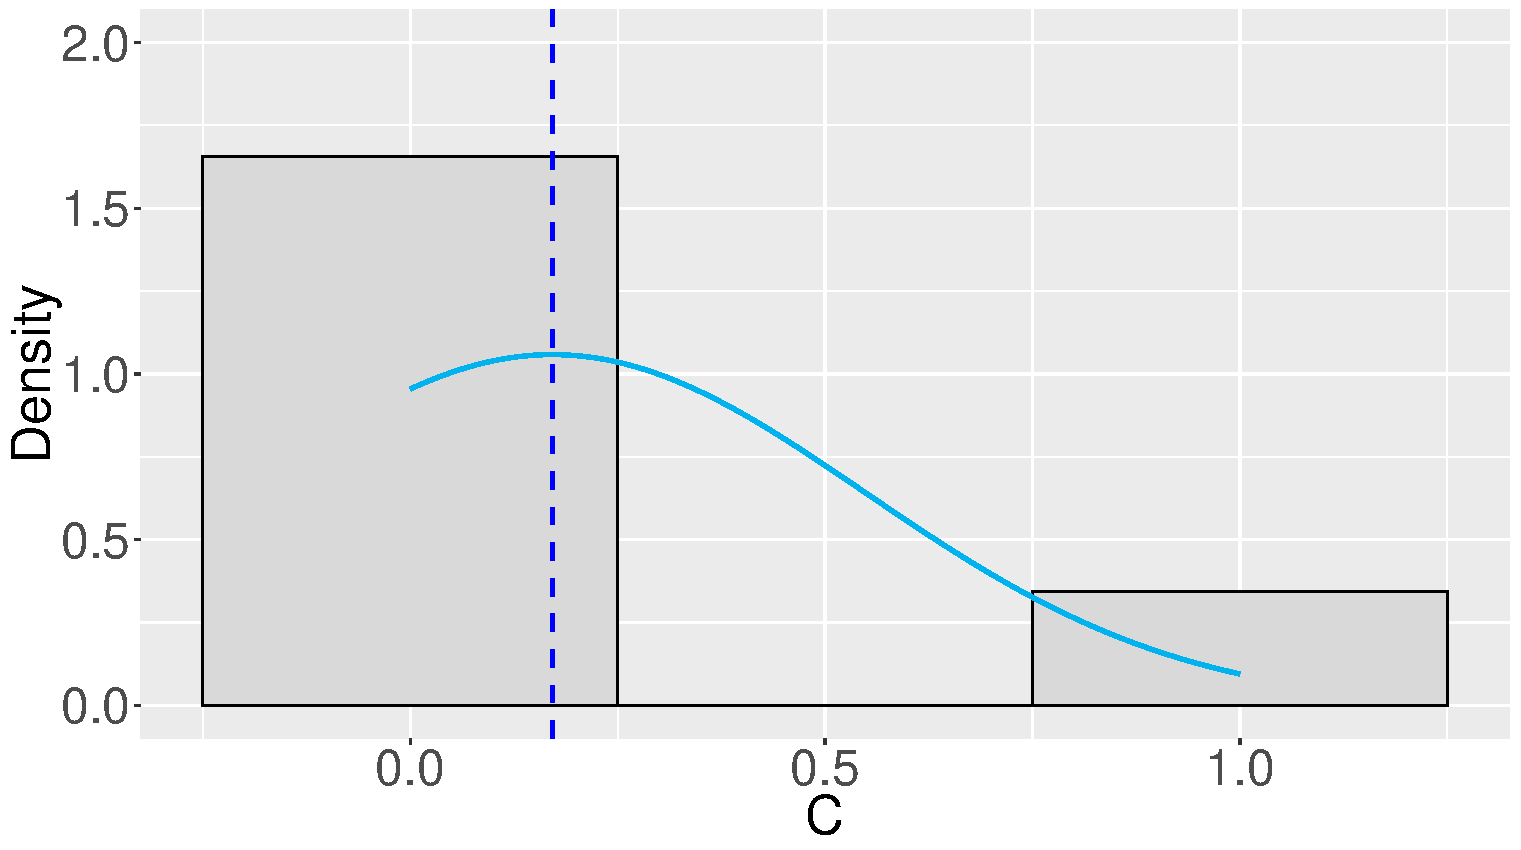
\includegraphics[width=2.9in]{CHist.pdf}
    \label{fig3.3:a}
  \end{subfigure}
  \begin{subfigure}[b]{0.5\linewidth}
    \centering
    \hspace{-13pt}
    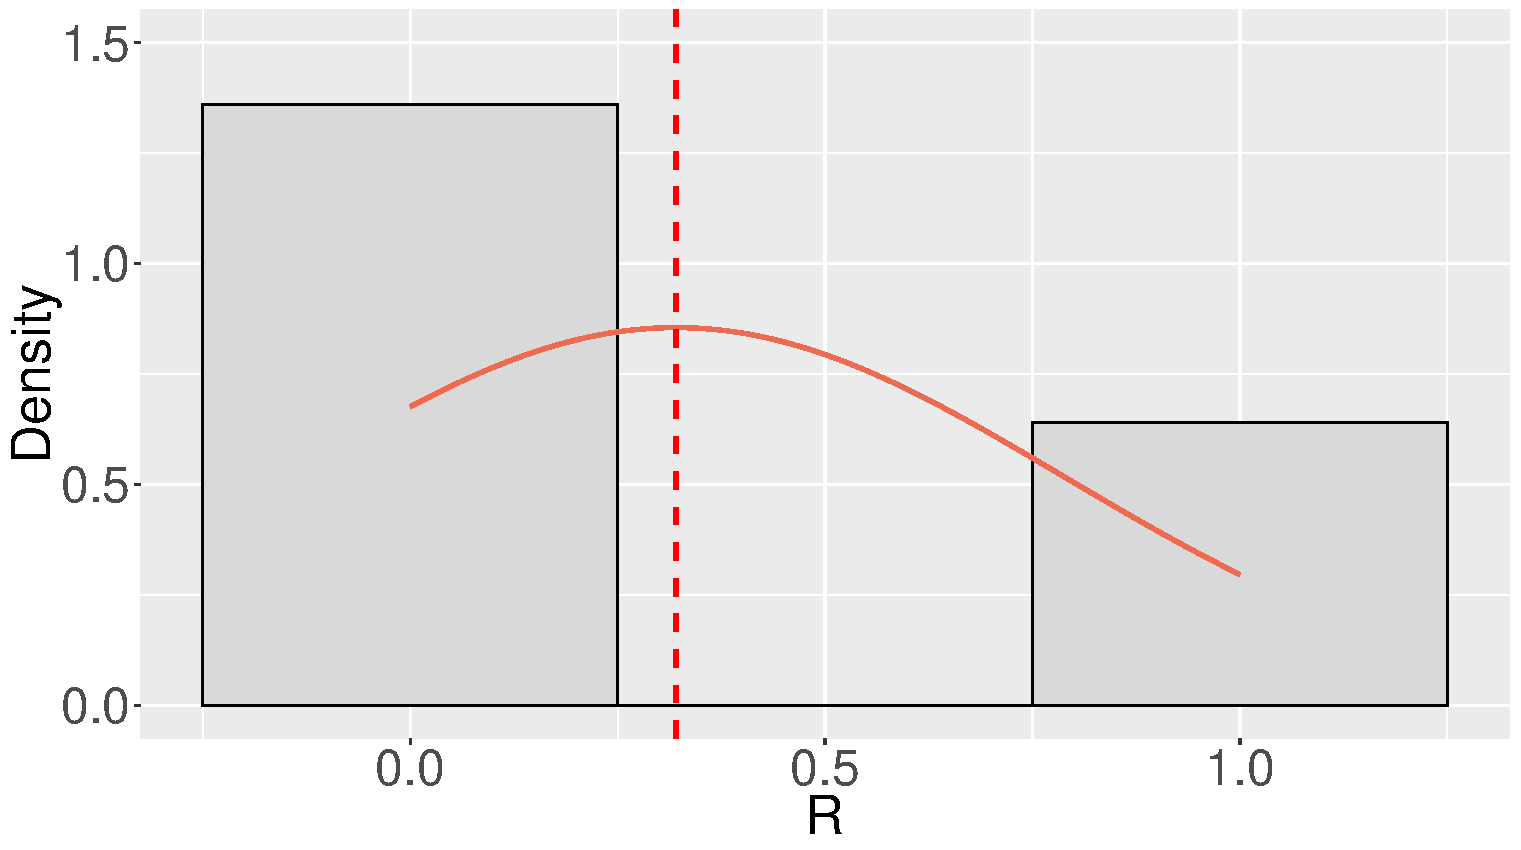
\includegraphics[width=2.9in]{RHist.pdf}
    \label{fig3.3:b}
  \end{subfigure}\hfill%
  \caption{These two graphs show the histogram along with thePDF and the mean value for parameters $C$ and $R$. The PDFs are plotted using solid lines and the means are plotted using dashed lines. Since they only take values True and False we must convert these to numerical values $1$ and $0$. This is the reason for there being only two levels of frequency.}
  \label{fig3.3} 
\end{figure}
These are the two posterior distributions for the probabilities $P(C)$ and $P(R)$. So, after only using the conditional probabilities, we have managed to apply Gibbs sampler and arrive at two unconditional probabilities of
\begin{align*}
P(C) &= 0.1715 \pm \sigma_C,\quad\sigma_C = 0.3770\\
P(R) &= 0.3204 \pm \sigma_R,\quad\sigma_R = 0.4667
\end{align*}
where $\sigma_{C,R}$ is the standard deviation. We can also give confidence intervals for these results. For a 95.8\% confidence interval we have
\begin{align*}
-0.5824 \leq &P(C) \leq 0.9254\\
-0.6129 \leq &P(R) \leq 1.2537
\end{align*}
Though having a probability less than zero or greater than 1 doesn't make much sense. Plotting the posterior distribution in Figure \ref{fig3.4} looks rather strange. There are only 4 points corresponding to the 4 possible states the two parameters can be. A very simplified version from Figure \ref{fig3.5}. This is also why so many iterations were required because the algorithm cannot converge to a single point in parameter space. 
\begin{figure}[H]
\centering
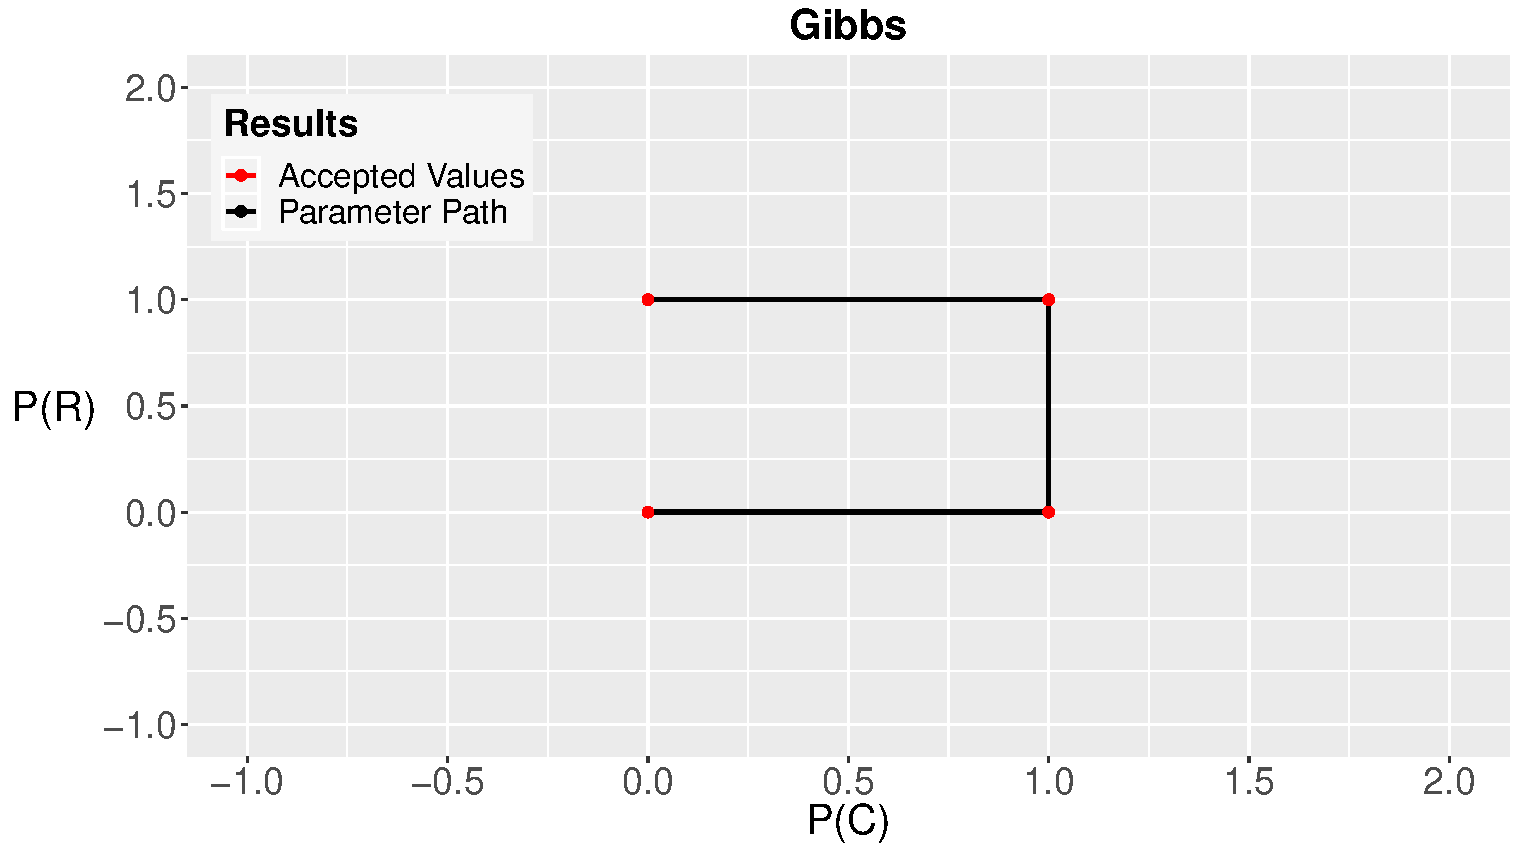
\includegraphics[width = 4.3in]{Gibbsfinal.pdf}
\caption{Plot of how the Gibbs algorithm moves through parameter space for both parameters. If I were to plot all the accepted values then we just have a unit square so I have restricted the data to the first 15 values. Within these 15 values the sampler moves from (1,1) to (0,1), back to (1,1), then to (1,0), and finally to (0,0).}
\label{fig3.4}
\end{figure}
It is hard to see the movement of the algorithm. The lines connecting each point overlap each other so all movements after the first few are hidden. 

(For the code used in this example visit this \href{https://github.com/iMikeT/MathProject2/tree/master/R%20Code/Gibbs/Bayesian%20Network%20Example}{link}.)

(See \cite{3} Chapter 14 for more detail on \S\ref{The Gibbs Sampler})

\chapter{Applications of Machine Learning}\label{Applications of Machine Learning}

We move on now from MCMC sampling for an estimate posterior PDF into the more in depth realm of machine learning. I have researched some different machine learning techniques and applied them to some examples. The machine learning process I have focused on is classification. The simplest technique for this is \bb{na\"{i}ve Bayes}.

\section{Na\"{i}ve Bayesian Algorithm}\label{Naive Bayesian Algorithm}
\vspace{-0.4in}
\underline{\hspace{6.2in}}
\vspace{-0.1in}

\bb{Na\"{i}ve Bayes Classifiers} are a group of probabilistic classifiers that use Bayes' Theorem to make a prediction for an outcome given some features, where these features are assumed to be \bb{strongly independent}. What is a classifier? It is a model that will assign a feature to a class based on observations. But what are features and classes? I'll explain in a moment.

A common application of a na\"{i}ve Bayes' classifier is binary classification. This means that there are only two classes. For example, we might want to classify if a fruit is an apple or an orange. Here the label would be fruit. A label is just a name given to the group of features, and the classes would be apple or orange. A possible feature for a classifier like this could be the colour of the fruit. So, if we have an orange fruit then we classify it as an orange. The more features we have, the more sophisticated the classifier becomes.

With a basic idea of what a classifier is, we can begin by looking at how this na\"{i}ve Bayes classification works. Since this classifier used Bayes' Theorem, it is a conditional probability model.
\begin{definition}\label{naive def}
\bb{Na\"{i}ve Bayes:} Given a list of labels, $(x_1,x_2,\ldots,x_n)$ where $n\in\N$ is the number of labels, it assigns the probability
\begin{align*}
P(C_k\mid x_1,x_2,\ldots,x_n),\quad k\in\N\,\text{ where }\,1\leq k\leq K
\end{align*}
Here $K$ is the number of classes. Using Bayes' Theorem, we can write
\begin{align}
P(C_k\mid x_1,x_2,\ldots,x_n) = \dfrac{P(C_k)\times P(x_1,x_2,\ldots,x_n\mid C_k)}{P(x_1,x_2,\ldots,x_n)}\label{4.1}
\end{align}
The numerator can also be regarded as the joint probability which can be written as
\begin{align*}
P(C_k,x_1,x_2,\ldots,x_n) = P(x_1,x_2,\ldots,x_n,C_k)
\end{align*}
Using the chain rule this expression can be expanded
\begin{align*}
P(x_1,x_2,\ldots,x_n,C_k) &= P(x_1\mid x_2,\ldots,x_n,C_k)P(x_2,x_3,\ldots,x_n,C_k)\\
&= P(x_1\mid x_2,\ldots,x_n,C_k)P(x_2\mid x_3,\ldots,x_n,C_k)P(x_3,x_4,\ldots,x_n,C_k)\\
&\hspace{6pt}\vdots\\
&= P(x_1\mid x_2,\ldots,x_n,C_k)\cdots P(x_{n-1}\mid x_n,C_k)P(x_n\mid C_k)P(C_k)
\end{align*}
Assume that all the labels $(x_1,x_2,\ldots,x_n)$ are \bb{independent}. This gives us
\begin{align*}
P(x_i\mid x_{i+1},x_{i+2},\ldots,x_n,C_k)\approx P(x_i\mid C_k)\,\text{ where }\,i=1,2,\ldots,n
\end{align*}
This means we can express the joint model as
\begin{align*}
P(C_k\mid x_1,x_2,\ldots,x_n) \approx \dfrac{P(C_k)\times P(x_1\mid C_k)\times P(x_2\mid C_k)\times\cdots\times P(x_n\mid C_k)}{P(x_1,x_2,\ldots,x_n)}
\end{align*}
Since the denominator does not depend on the class $C$ it will not change and can be considered a constant. If the denominator is  omitted this gives us the following proportionality relation
\begin{align}
P(C_k\mid x_1,x_2,\ldots,x_n) \propto P(C_k)\prod^n_{i=1}P(x_i\mid C_k)\label{4.2}
\end{align}
We have derived a final expression for the conditional probability model to be used in the classifier. The final stage is to use this expression to define a decision rule, which will decide the class $C_k$ that the labels $(x_1,x_2,\ldots,x_n)$ belong to. This is know as the \bb{maximum a posteriori} which works by assigning the label to the class where the conditional probability product, $P(C_k)\prod^n_{i=1}P(x_i\mid C_k)$ is greatest. This is given by
\begin{align*}
\hat{C} = \argmax_{k\in\{1,\ldots,K\}}P(C_k)\prod^n_{i=1}P(x_i\mid C_k)
\end{align*}
\end{definition}

The reason why this classifier has its name is due to the assumption we made that all the labels and features are \bb{independent}. In the real world this is not always the case. Some might not be independent, making the final answer \ti{na\"{i}ve}. But, when applied to the right problem, the na\"{i}ve Bayes classifier still performs well.

\section{Binary Classification}\label{Binary Classification}
\vspace{-0.4in}
\underline{\hspace{6.2in}}
\vspace{-0.1in}

Here we have the number of classes $K = 2$. This is most common with scenarios where the answer is yes or no. We will apply the definition of na\"{i}ve Bayes to an example of binary classification.

\subsection{To Play or not to Play}\label{play example}
\vspace{-0.35in}
\underline{\hspace{6.2in}}
\vspace{-0.1in}

Suppose we want to classify if a baseball team will play, depending on the weather. So the label would be \ti{Weather} comprised of the features \ti{Sunny}, \ti{Overcast} and \ti{Rain}, and the classes are \ti{Yes} (the team played) and \ti{No} (the team did not play). We have some observational data for the past few days where the weather was recorded and if the team played baseball, which will then be used to calculate the conditional probabilities needed to perform a na\"{i}ve Bayes classification.

A keen observation can be made here. Since we only have one label \ti{Weather}, equation (\ref{4.1}) breaks down to the ordinary Bayes' Theorem we all know and love. Making these calculations the simplest ones possible for a na\"{i}ve Bayes classification. For the data used in this example see \ref{tab:play} of Appendix A. So now we can create problems for the classifier to process.

For example, will the team play if it is raining? We need to calculate the probability of the classes given that it is raining. So, the probability that the team will play (class Yes) is given by
\begin{align*}
P(\text{Yes}\mid\text{Rain}) = \dfrac{P(\text{Rain}\mid \text{Yes})\times P(\text{Yes})}{P(\text{Rain})}
\end{align*}
To calculate this we need
\begin{align*}
P(\text{Rain}) = \frac{5}{14} = 0.3571,\quad P(\text{Yes}) = \frac{9}{14} = 0.6429,\quad P(\text{Rain}\mid \text{Yes}) = \frac{2}{9} = 0.2222
\end{align*}
Substituting this into the equation gives
\begin{align*}
P(\text{Yes}\mid\text{Rain}) = \dfrac{0.2222\times 0.6429}{0.3571} = 0.4
\end{align*}
We then perform the same process for the probability that the team will not play (class No) resulting in
\begin{align*}
P(\text{No}\mid\text{Rain}) = \dfrac{P(\text{Rain}\mid \text{No})\times P(\text{No})}{P(\text{Rain})} = \dfrac{0.6\times 0.3571}{0.3571} = 0.6
\end{align*}
So we have that
\begin{align*}
P(\text{No}\mid\text{Rain}) > P(\text{Yes}\mid\text{Rain})
\end{align*}
Thus, the decision rule would choose the class No. In plain English this means that if it is raining then the team will not play ball. When I first saw this, I was amazed. By only using observed data and Bayes' Theorem, we can predict what the outcome will be for a given condition.

Notice how the denominator is the same in both classes? This is what was mentioned at the end of definition \ref{naive def}. It is not dependent on the current class so it will remain the same for all classes. Like before, it is just a normalising term that makes the probabilities add up to 1. If we had of omitted the denominator term in both then we would still have the same outcome that the team will not play ball as
\begin{align*}
P(\text{Yes}\mid\text{Rain}) &\propto 0.2222\times 0.6429 = 0.1429\\
P(\text{No}\mid\text{Rain}) &\propto 0.6\times 0.3571 = 0.2143
\end{align*}
What we have just done with basic statistics is machine learning! Now granted, this is a basic level but it still counts. To illustrate the more general process we can add more labels to this example.

\subsection{Is It Too Hot, or Too Cloudy, or Both to Play Ball?}\label{temp example}
\vspace{-0.35in}
\underline{\hspace{6.2in}}
\vspace{-0.1in}

We will be using the same example and problem as in \S\ref{play example} but with the extra label \ti{Temperature}. So now we have the label \ti{Weather} consisting of the features \ti{Sunny}, \ti{Overcast}, and \ti{Rain}, and the label \ti{Temperature} consisting of the features \ti{Hot}, \ti{Mild}, and \ti{Cool}. For the data used in this example see \ref{tab:temp} of Appendix A.

For example, will the team play if it is overcast and it is hot? To calculate this we will use equation (\ref{4.2}) now that we have two labels ($n = 2$). So, the probability that the team will play is given by
\begin{align*}
P(\text{Yes}\mid \te{Overcast}, \te{Hot}) &\propto P(\te{Yes})\times P(\te{Overcast},\te{Hot}\mid\te{Yes})\\
&= P(\te{Yes})\times P(\te{Overcast}\mid\te{Yes})\times P(\te{Hot}\mid\te{Yes})\\
&= 0.6429 \times 0.4444 \times 0.2222 = 0.0635
\end{align*}
and the probability that the team will not play is given by
\begin{align*}
P(\text{No}\mid \te{Overcast}, \te{Hot}) &\propto P(\te{No})\times P(\te{Overcast},\te{Hot}\mid\te{No})\\
&= P(\te{No})\times P(\te{Overcast}\mid\te{No})\times P(\te{Hot}\mid\te{No})\\
&= 0.3571 \times 0 \times 0.4 = 0
\end{align*}
So we have that
\begin{align*}
P(\text{Yes}\mid\te{Overcast}, \te{Hot}) > P(\text{No}\mid\te{Overcast}, \te{Hot})
\end{align*}
So this time the decision rule predicts the team will play ball! Hopefully it is not too hot. If it is then machine learning computer does not care. Now we can look into how a process like na\"{i}ve Bayes is implemented through a computer. If we had dozens of labels then doing this by hand would not be difficult but extremely tedious. That is where Python comes into play.

\subsection{Scikit-Learn}\label{Scikit-learn}
\vspace{-0.35in}
\underline{\hspace{6.2in}}
\vspace{-0.1in}

Scikit-learn have a range of unsupervised and supervised machine learning algorithms all bundled into one Python package. This makes it the perfect tool to use for the machine learning purposes I will cover. We can use the same data from section \S\ref{temp example} and place it into the Scikit-learn process.

The main challenge with machine learning is not the calculations but preparing the data. Here we have data given in words and for scikit to process this we need to convert them to numbers. This can be done using function called \colorbox{codegrey}{\texttt{label encoder}}. Running this for the two labels \colorbox{codegrey}{\texttt{Weather}} and \colorbox{codegrey}{\texttt{Temperature}}, and the class \colorbox{codegrey}{\texttt{Play}} we have the following
\begin{align*}
\texttt{Weather: [2 2 0 1 1 1 0 2 2 1 2 0 0 1],}&\texttt{ 0:Overcast, 1:Rain, 2:Sunny}\\
\texttt{Temperature: [1 1 1 2 0 0 0 2 0 2 2 2 1 2],}&\texttt{ 0:Cool, 1:Hot, 2:Mild}\\
\texttt{Play: [0 0 1 1 1 0 1 0 1 1 1 1 1 0],}&\texttt{ 0:No, 1:Yes}
\end{align*}
Looking back at \ref{tab:temp} we see what each number corresponds to in each label and class.

Next is to link the features of \colorbox{codegrey}{\texttt{Weather}} and \colorbox{codegrey}{\texttt{Temperature}} together into one variable, resulting in a list of tuples. Even though the choosing of which number goes to which feature is done alphabetically, the original order of the data is preserved. So we can just group up the two as they are. I have chosen to call this variable \colorbox{codegrey}{\texttt{Label}}
\begin{align*}
\texttt{Label: [}&\texttt{(2, 1), (2, 1), (0, 1), (1, 2), (1, 0), (1, 0), (0, 0),}\\
&\texttt{(2, 2), (2, 0), (1, 2), (2, 2), (0, 2), (0, 1), (1, 2)]}
\end{align*}
Lastly, we are ready in perform na\"{i}ve Bayes classification, just as we did before by hand, through Scikit. One technical note, Scikit na\"{i}ve Bayes classifiers need to be given an assumption about how $P(x_i\mid C_k)$ is distributed in equation (\ref{4.2}). So to get this classifier working we will choose the most basic \ti{Gaussian} na\"{i}ve Bayes given as
\begin{align*}
P(x_i\mid C_k) = \dfrac{1}{\sqrt{2\pi\sigma^2_{C_k}}}\cdot\exp\bkt{-\dfrac{(x_i - \mu_{C_k})^2}{2\sigma^2_{C_k}}}
\end{align*}
where $\sigma^2_{C_k}$ and $\mu_{C_k}$ are estimated using maximum likelihood. So, for this example, the likelihood of the labels is assumed to be normally distributed. It's just an assumption we have made that won't affect the process very much. The code is simple to write, using the function \colorbox{codegrey}{\texttt{GaussianNB}}, as
\begin{align*}
&\texttt{model = GaussianNB()}\\
&\texttt{model.fit(Label,Play)}\\
&\texttt{predicted = model.predict([[0,1]])}
\end{align*}
where \colorbox{codegrey}{\texttt{0:Overcast}} and \colorbox{codegrey}{\texttt{1:Hot}}. We grouped the features in the order \colorbox{codegrey}{\texttt{Weather}} then \colorbox{codegrey}{\texttt{Temperature}} so that is the order they need to be entered into \colorbox{codegrey}{\texttt{model.predict()}}. Running this code gives the output
\begin{align*}
&\texttt{predicted = 1}
\end{align*}
which we know for \colorbox{codegrey}{\texttt{Play}} is a \colorbox{codegrey}{\texttt{Yes}}. We have the same result we calculated by hand (which is reassuring). Because the dataset is so small (14 observations), the classifier will not be very accurate. If we had more data then the classifier would be more reliable.

This concludes machine learning for binary classification! We gave a machine some data and it made a prediction on the outcome for given features. Furthermore, we now understand \ti{how} the machine used na\"{i}ve Bayes to calculate the different probabilities and select the greatest one as the prediction. 

I would next like to cover an example application of machine learning that is performed for everyone without even realising it. Have you ever opened you emails and seen that you have junk emails? How does your email service know that these emails are junk? The truth is that these emails are being classified using a machine learning technique. They could be using na\"{i}ve Bayes algorithm or another form of classification. Lets see how a process like this would work.

(For the code used in this example visit this \href{https://github.com/iMikeT/MathProject2/tree/master/Python%20Code/Baseball%20Classification}{link}.)

\subsection{Politics or Sports}\label{sports example}
\vspace{-0.35in}
\underline{\hspace{6.2in}}
\vspace{-0.1in}

We are going to build a classifier to predict if a sentence is about politics or sports. Suppose we have the following dataset given in \ref{tab:text} of Appendix A and we want to predict if the sentence ``A very close game'' is about sports or politics. Obviously this is about sports but can the classifier get it right?

The way to do this is by adding the sentence to the dataset and using the first 5 as training data and the last sentence as testing data. Because we are working with text we need to remove the capitalization so ``A'' and ``a'' are not treated as two different words. Then we need to encode this data like before by dividing the sentences into individual words.

There are 14 words in total so each word will be encoded from \colorbox{codegrey}{\texttt{0}} to \colorbox{codegrey}{\texttt{13}} and the number of labels is the number of words in the sentence to be classified. This is why we enter the sentence into the dataset as calling it through numbers would be confusing. lastly, we set split the training and test data as
\begin{align*}
&\texttt{N = 6}\\
&\texttt{n = N-1}\\
&\texttt{X\_train = Data[`Text'][:n]}\\
&\texttt{Y\_train = Data[`Tag'][:n]}\\
&\texttt{X\_test = Data[`Text'][n:N]}\\
&\texttt{Y\_test = Data[`Tag'][n:N]}\\
\end{align*}
where \colorbox{codegrey}{\texttt{N}} is the number of sentences. We train up to the 5$^\text{th}$ sentence and test the last one. To do this example by hand, the probabilities are calculated in the same way as \S\ref{temp example}. To find these you would need to exclude the last sentence from the dataset as that's the one we are now working with. It would look like the following
\begin{align*}
P(\text{Sports}\mid \te{a}, \te{very}, \te{close}, \te{game}) &\propto P(\te{Sports})\times P(\te{a}, \te{very}, \te{close}, \te{game}\mid\te{Sports})\\
&= P(\te{Sports})\times P(\te{a}\mid\te{Sports})\times P(\te{very}\mid\te{Sports})\times\\
&\quad\,\,P(\te{close}\mid\te{Sports})\times P(\te{game}\mid\te{Sports})\\
&= \frac{3}{5} \times \frac{2}{11} \times \frac{1}{11} \times \frac{0}{11} \times \frac{2}{11} = 0
\end{align*}
This isn't good. The word ``close'' does not appear in the Sports text, which is giving us a zero result. This means that we are losing all the information from the other probabilities. The workaround for this issue is known as \bb{Laplace smoothing} where we just add one to every word count so that there is never a zero probability in the calculation. And to balance this increase, we add the total number of words to the denominators so the probabilities will never be greater than 1. Doing this gives
\begin{align*}
P(\text{Sports}\mid \te{a}, \te{very}, \te{close}, \te{game}) &\propto \frac{3}{5} \times \frac{2+1}{11+14} \times \frac{1+1}{11+14} \times \frac{0+1}{11+14} \times \frac{2+1}{11+14}\\
&= \frac{3}{5} \times \frac{3}{25} \times \frac{2}{25} \times \frac{1}{25} \times \frac{3}{25} = 2.7648\times10^{-5}
\end{align*}
Repeating for the class Politics, and using Laplace smoothing again since ``very'' and ``game'' are would give zero conditional probabilities, gives
\begin{align*}
P(\text{Politics}\mid \te{a}, \te{very}, \te{close}, \te{game}) &\propto P(\te{Politics})\times P(\te{a}, \te{very}, \te{close}, \te{game}\mid\te{Politics})\\
&= P(\te{Politics})\times P(\te{a}\mid\te{Politics})\times P(\te{very}\mid\te{Politics})\times\\
&\quad\,\,P(\te{close}\mid\te{Politics})\times P(\te{game}\mid\te{Politics})\\
&= \frac{2}{5} \times \frac{1+1}{9+14} \times \frac{0+1}{9+14} \times \frac{1+1}{9+14} \times \frac{0+1}{9+14}\\
&= \frac{2}{5} \times \frac{2}{23} \times \frac{1}{23} \times \frac{2}{23} \times \frac{1}{23} = 5.7175\times10^{-6}
\end{align*}
At last we have the conclusion that
\begin{align*}
P(\text{Sports}\mid \te{a}, \te{very}, \te{close}, \te{game}) > P(\text{Politics}\mid \te{a}, \te{very}, \te{close}, \te{game})
\end{align*}
so we would choose that the sentence ``A very close game'' is about Sports. Huzza! We have a correct prediction from the classifier. Running the Python code using scikit for the same sentence gives the result
\begin{align*}
\texttt{predicted = [`Sports']}
\end{align*}
So we know the classifier in Python is working correctly since we checked the mathematics.  Although, there is an interesting issue that depends on the sentence you choose to classify. For example, If we wanted to classify the sentence ``Not a violent debate'', we know this is about Politics but the only word in this sentence that is in the training data is ``a''. Even with the Laplace smoothing, we would have that
\begin{align*}
P(\text{Sports}\mid \te{not}, \te{a}, \te{violent}, \te{debate}) &\propto P(\te{Sports})\times P(\te{a}\mid\te{Sports})\times\cdots\\
&= \frac{3}{5}\times\frac{3}{25}\times\frac{1}{25^3} = 4.608\times10^{-6},\\
\end{align*}
\vspace{-25pt}
\begin{align*}
P(\text{Politics}\mid \te{not}, \te{a}, \te{violent}, \te{debate}) &\propto P(\te{Politics})\times P(\te{a}\mid\te{Politics})\times\cdots\\
&= \frac{2}{5}\times\frac{2}{23}\times\frac{1}{23^3} = 2.859\times10^{-6}.\\
\end{align*}
So this is why running the Python code with the sentence ``Not a violent debate'' is incorrectly classified as
\begin{align*}
\texttt{predicted = [`Sports']}
\end{align*}
One counter measure to this is removing stopwords such as ``a'', ``else'', ``ever'', words that don't add information but we would still have the incorrect answer of sports since
\begin{align*}
\frac{3}{5}\times\frac{1}{25^3} = 3.84\times10^{-5} > 3.29\times10^{-5} = \frac{2}{5}\times\frac{1}{23^3}
\end{align*}
We simply need to have more data to make the classifier more reliable. Which is why the larger the dataset, the better the machine learning result. We can try some other sentences for fun and see the results from the code. I will put them in a table below
\begin{table}[H]
  \centering
  \begin{tabular}{|c|c|}
    \hline
    Sentence & Prediction\\
\hline
Voting time is over & \texttt{[`Politics']}\\
The election result was tampered with & \texttt{[`Politics']}\\
A forgettable election & \texttt{[`Politics']}\\
It is a great game & \texttt{[`Sports']}\\
That is a touchdown & \texttt{[`Sports']}\\
Homerun & \texttt{[`Sports']}\\
\hline
It is a homerun & \texttt{[`Politics']}\\
\hline
  \end{tabular}
\end{table}
Adding all of these correct predictions to the dataset would improve its accuracy even more. We were lucky with the last two correct sports predictions as none of the words are in the training data so they were given the class Sport purely from the above calculation.

The last sentence is given the wrong prediction \colorbox{codegrey}{\texttt{[`Politics']}} because of the word ``it''. But if we update the training data with ``It is a great game'' being Sports, then we have
\begin{align*}
\texttt{It is a homerun = [`Sports']}
\end{align*}
The main flaw is with the dataset. We have that when no words are used in training, we get Sports. A simple fail safe could be added where the program asks for the classification of a sentence to be given when there are no known words.

Please view the Python code that I have written for this example. It took much time and careful programming to achieve. I would like to discuss the inner workings of the code more but feel that it would be too complicated for those who are not familiar with Python. So I will leave a link to the code for viewing on my GitHub repository.

(For the code used in this example visit this \href{https://github.com/iMikeT/MathProject2/tree/master/Python%20Code/Text%20Classification}{link}.)

(See \cite{4} for more detail on \S\ref{Naive Bayesian Algorithm} and \S\ref{Binary Classification})

\section{Multiple Classification}\label{Multiple Classification}
\vspace{-0.4in}
\underline{\hspace{6.2in}}
\vspace{-0.1in}

We have spent time with binary classification so lets take what has been covered here into the more interesting \bb{multiple classification}. This is when the number of classes $K\geq3$. Taking everything coved through \S\ref{Naive Bayesian Algorithm}-\S\ref{Scikit-learn}, we will tackle another example using Scikit.

\subsection{Is This Wine Locally Sourced}\label{wine example}
\vspace{-0.35in}
\underline{\hspace{6.2in}}
\vspace{-0.1in}

For this example I am using a famous multi-class classification problem involving wine. The dataset is available at the following \href{https://archive.ics.uci.edu/ml/datasets/wine}{link}. The data is for wines grown in the dame region in Italy but derived from three different cultivars. This is much more technically challenging because the dataset is much larger than the previous ones so I will only tackle this example using Python.

The dataset is loaded into Python through scikit as
\begin{align*}
&\texttt{from sklearn import datasets}\\
&\texttt{wine = datasets.load\_wine()}
\end{align*}

Exploring the dataset will tell us more about the features, labels and classes. Here there is one label \colorbox{codegrey}{\texttt{Wine}} and 13 different features each with 178 values, and three different classes. We will use na\"{i}ve Bayes to predict what class a wine belongs to given its 13 different feature values. Lets see how this looks
\begin{align*}
\texttt{Features: [}&\texttt{`alcohol', `malic\_acid', `ash', `alcalinity\_of\_ash',}\\
&\texttt{`magnesium', `total\_phenols', `flavanoids',}\\
&\texttt{`nonflavanoid\_phenols', `proanthocyanins', `color\_intensity',}\\
&\texttt{`hue', `od280/od315\_of\_diluted\_wines', `proline']}\\
\texttt{Class: [}&\texttt{`class\_0' `class\_1' `class\_2'}
\end{align*}
That is a lot of different features. Who knew that wine could be so complicated! If we view the first row of the dataset we see that the data is given in decimals so there is no feature encoding needed this time
\begin{align*}
\texttt{[[ }&\texttt{1.42300000e+01  1.71000000e+00  2.43000000e+00  1.56000000e+01}\\
&\texttt{1.27000000e+02   2.80000000e+00   3.06000000e+00   2.80000000e-01}\\
&\texttt{2.29000000e+00   5.64000000e+00   1.04000000e+00   3.92000000e+00}\\
&\texttt{1.06500000e+03]]}
\end{align*}
The double brackets here are because the data is stored in one vector comprised of 178 vectors each with 13 elements for each feature. The first row is just 1 of the 178 vectors. Now, for each of these vectors, we know which class it belongs to. Just like how we knew if the baseball team played or not for the 14 observations is \S\ref{Scikit-learn}.

The next crucial step is called \bb{splitting the data}. This is for testing the accuracy of the na\"{i}ve Bayes classifier. We will have a portion of the dataset for training and the rest for testing. This can all be performed in scikit with a single line of code using the \colorbox{codegrey}{\texttt{train\_test\_split}} function
\begin{align*}
\texttt{X\_train, X\_test, y\_train, y\_test = }&\texttt{train\_test\_split(wine.data, wine.target,}\\
&\texttt{test\_size=0.3,random\_state=x)}
\end{align*}
where the \colorbox{codegrey}{\texttt{X}} variables are the feature data and the \colorbox{codegrey}{\texttt{y}} variables are the class data. The \colorbox{codegrey}{\texttt{test\_size=0.3}} argument means that 30\% of the dataset will be used for testing so the remaining 70\% is used for training. \colorbox{codegrey}{\texttt{random\_state=x}} is for a random number generator where, for a positive integer \colorbox{codegrey}{\texttt{x}}, the random numbers will be the same for consistency in testing so that the classes and the associated feature values are all mixed up. Lets choose \colorbox{codegrey}{\texttt{x = 32}}. Then, we do the same as we did before
\begin{align*}
&\texttt{model = GaussianNB()}\\
&\texttt{model.fit(X\_train,y\_train)}\\
&\texttt{predicted = model.predict(X\_test)}
\end{align*}
To then calculate the accuracy we use scikit \colorbox{codegrey}{\texttt{metrics}} module
\begin{align*}
\texttt{Accuracy }&\texttt{= metrics.accuracy\_score(y\_test, predicted))}\\
&\texttt{= 0.9$\overline{\texttt{814}}$}
\end{align*}
So the Gaussian na\"{i}ve Bayes predictions were 98.1\% correct. But sometimes the classifier would perform better depending on the value of \colorbox{codegrey}{\texttt{random\_state}}. So I performed a loop where the classifier would run 50 times with a different \colorbox{codegrey}{\texttt{random\_state}} value each time going from \colorbox{codegrey}{\texttt{x = 1,2,3,...,50}} and take the average of all these percentages. 

I would then repeat this process for different values of \colorbox{codegrey}{\texttt{test\_size}} and plot the results to visualise how increasing the training size makes the classifier perform better in Figure \ref{fig4.2}. The more data that the classifier has to train with, the \ti{smarter} it becomes. After training size = 40\% the machine learning process is not really \ti{learning} any more.

We see the average accuracy percentage start to level out. This is good to note because at training size = 40\% the average percentage accuracy is 96.53211\%. If this was accurate enough for some hypothetical purposes then we would not need to continue training the classifier, essentially making the process more efficient.
\begin{figure}[H]
\centering
\includegraphics[width = 4.3in]{GaussianNB.png}
\caption{Plot of the average accuracy for the Gaussian na\"{i}ve Bayes classifier for the percentage of dataset used for training. It takes the form of the logarithmic progression. Before even using just 20\% of the data as training we already have an average accuracy greater than 80\%.}
\label{fig4.2}
\end{figure}

(For the code used in this example visit this \href{https://github.com/iMikeT/MathProject2/tree/master/Python%20Code/Wine%20Classification}{link}.)

\section*{Conclusions}
\vspace{-0.4in}
\underline{\hspace{6.2in}}
\vspace{-0.1in}

Working with MCMC algorithms and machine learning methods, I have gained the skills to apply statistical mathematics to real world problems. After reading this report you should have a complete understanding on:
\begin{itemize}
\item Why performing analytical calculations using Bayes theorem is not always possible and why the posterior is proportional to the un-normalised posterior.
\item The Metropolis algorithm and how the acceptance ratio calculates the probability that the next sample value is accepted or rejected.
\item The Metropolis-Hastings algorithm and its modification that prevents potential samples being lost due parameter boundaries by allowing asymmetric proposal distributions.
\item The Gibbs algorithm and its ability to accept all proposed samples, allowing for faster convergence to the posterior distribution.
\item Using a Bayesian network and applying Gibbs algorithm to sample from the different conditional probabilities to give estimates on unconditional probabilities.
\item The mathematics of the na\"{i}ve Bayes classification algorithm and its application in everyday life.
\item Why a machine learning algorithms accuracy is proportional the the amount of data it has to learn from.
\end{itemize}

What I would do given more time is an introduction into the mathematics of neural network. These are used for much more complicated classification such as finding patterns in handwriting. I also wanted to formulate a problem where all sampling algorithms could be applied and compare the rate of convergence for each. Depending on the severity of correlation between the parameters would determine which algorithms would converge the fastest. I will still go on to learn more about neural networks after my project because of my vast interest in the subject. It is the gateway to the future and we must tread with caution.

\chapter*{Acknowledgements}

This work would not have been possible without the support of everyone involved.

I am especially indebted to Dr. Siri Chongchitnan, who has worked actively to provide me with guidance and support throughout my four year Master of Mathematics degree.

Thank you to my Mother and Father, Christina Turner and Leonard Turner, for working hard to proofread this report and for always encouraging me to be the best I can be.

Thank you to my Auntie, Diane Greening, for your constant care and being the person in my life who introduced me to the world of science. Enrolling in a mathematics degree might never have happened without your influence.

Thank you to my Partner, Rebecca Baker. We have made it through university only because of the daily love and support we give one another. I will always be thankful to have you in my life.

Thank you to my Sister, Kerri-Marie Turner, for always believed in me growing up.

And finally, thank you to my Grandmother, Kathleen Greening, for taking care of me throughout the years from primary school to university.

\bibliographystyle{unsrt}
\bibliography{Ref}
\pagebreak

\pagestyle{plain}
\appendix
\chapter{Tables}

\begin{table}[H]
  \centering
  \caption{Data table for the weather and the play outcome, the frequency table for the weather, the likelihood table for the overall probabilities for weather and play, and the posterior probabilities table for Play. Here ``PP'' stands for Posterior Probability.}
  \label{tab:play}
    \begin{tabular}{|c|c|}
    \hline
    Weather & Play \\
\hline
Sunny & No\\
Sunny & No\\ 
Overcast & Yes\\
Rain & Yes\\
Rain & Yes\\
Rain & No\\
Overcast & Yes\\
Sunny & No\\
Sunny & Yes\\
Rain & Yes\\
Sunny & Yes\\
Overcast & Yes\\
Overcast & Yes\\
Rain & No\\
    \hline
  \end{tabular}
  \quad
  \begin{tabular}{|c|c|c|}
    \hline
    Weather & Yes & No \\
\hline
Overcast & 4 & 0\\
Sunny & 3 & 2\\ 
Rain & 2 & 3\\
\hline
Total & 9 & 5\\
    \hline
  \end{tabular}
\end{table}
\begin{table}[H]
  \centering
  \begin{tabular}{|c|c|c|c|c|}
    \hline
    Weather & Yes & No & Total & Weather Probability\\
\hline
Overcast & 4 & 0 & 4 & $4/14=0.2857$\\
Sunny & 3 & 2 & 5 & $5/14=0.3571$\\ 
Rain & 2 & 3 & 5 & $5/14=0.3571$\\
\hline
Total & 9 & 5 & 14 &\\
\hline
Play Probability & $9/14=0.6429$ & $5/14=0.3571$ &&\\
    \hline
  \end{tabular}
\end{table}
\begin{table}[H]
  \centering
  \begin{tabular}{|c|c|c|c|c|}
    \hline
    Weather & Yes & No & PP of Yes & PP of No\\
\hline
Overcast & 4 & 0 & $4/9=0.4444$ & $0/5=0$\\
Sunny & 3 & 2 & $3/9=0.3333$ & $2/5=0.4$\\ 
Rain & 2 & 3 & $2/9=0.2222$ & $3/5=0.6$\\
\hline
Total & 9 & 5 &&\\
    \hline
  \end{tabular}
\end{table}

\begin{table}[H]
  \centering
  \caption{Data table for the weather, temp and play, frequency table for the weather and the temp, the likelihood table for the overall probabilities for weather and play, and temp and play, and the posterior probabilities tables for play for weather and temp.}
  \label{tab:temp}
    \begin{tabular}{|c|c|c|}
    \hline
    Weather & Temperature & Play \\
\hline
Sunny & Hot & No\\
Sunny & Hot & No\\ 
Overcast & Hot & Yes\\
Rain & Mild & Yes\\
Rain & Cool & Yes\\
Rain & Cool & No\\
Overcast & Cool & Yes\\
Sunny & Mild & No\\
Sunny & Cool & Yes\\
Rain & Mild & Yes\\
Sunny & Mild & Yes\\
Overcast & Mild & Yes\\
Overcast & Hot & Yes\\
Rain & Mild & No\\
    \hline
  \end{tabular}
  \quad
  \begin{tabular}{|c|c|c|}
    \hline
    Weather & Yes & No \\
\hline
Overcast & 4 & 0\\
Sunny & 3 & 2\\ 
Rain & 2 & 3\\
\hline
Total & 9 & 5\\
    \hline
  \end{tabular}
  \quad
  \begin{tabular}{|c|c|c|}
    \hline
    Temp & Yes & No \\
\hline
Hot & 2 & 2\\
Mild & 4 & 2\\ 
Cool & 3 & 1\\
\hline
Total & 9 & 5\\
    \hline
  \end{tabular}
\end{table}
\begin{table}[H]
  \centering
  \begin{tabular}{|c|c|c|c|c|}
    \hline
    Weather & Yes & No & Total & Weather Probability\\
\hline
Overcast & 4 & 0 & 4 & $4/14=0.2857$\\
Sunny & 3 & 2 & 5 & $5/14=0.3571$\\ 
Rain & 2 & 3 & 5 & $5/14=0.3571$\\
\hline
Total & 9 & 5 & 14 &\\
\hline
Play Probability & $9/14=0.6429$ & $5/14=0.3571$ &&\\
    \hline
  \end{tabular}
\end{table}
\begin{table}[H]
  \centering
  \begin{tabular}{|c|c|c|c|c|}
    \hline
    Temp & Yes & No & Total & Temp Probability\\
\hline
Hot & 4 & 0 & 4 & $4/14=0.2857$\\
Mild & 3 & 2 & 6 & $6/14=0.4286$\\ 
Cool & 2 & 3 & 4 & $4/14=0.2857$\\
\hline
Total & 9 & 5 & 14 &\\
\hline
Play Probability & $9/14=0.6429$ & $5/14=0.3571$ &&\\
    \hline
  \end{tabular}
\end{table}
\begin{table}[H]
  \centering
  \begin{tabular}{|c|c|c|c|c|}
    \hline
    Weather & Yes & No & PP of Yes & PP of No\\
\hline
Overcast & 4 & 0 & $4/9=0.4444$ & $0/5=0$\\
Sunny & 3 & 2 & $3/9=0.3333$ & $2/5=0.4$\\ 
Rain & 2 & 3 & $2/9=0.2222$ & $3/5=0.6$\\
\hline
Total & 9 & 5 &&\\
    \hline
  \end{tabular}
\end{table}
\begin{table}[H]
  \centering
  \begin{tabular}{|c|c|c|c|c|}
    \hline
    Temp & Yes & No & PP of Yes & PP of No\\
\hline
Hot & 2 & 2 & $2/9=0.2222$ & $2/5=0.4$\\
Mild & 4 & 2 & $4/9=0.4444$ & $2/5=0.4$\\ 
Cool & 3 & 1 & $3/9=0.3333$ & $1/5=0.2$\\
\hline
Total & 9 & 5 &&\\
    \hline
  \end{tabular}
\end{table}
\begin{table}[H]
  \centering
  \caption{Data table for the text and tag, and splitting text and adding test text, and the frequency tables for the text, text in Sports, and text in Politics before adding test text.}
  \label{tab:text}
  \begin{tabular}{|c|c|}
    \hline
    Text & Tag\\
\hline
A great game & Sports\\
The election was over & Politics\\ 
Very clean match & Sports\\
A clean but forgettable game & Sports\\
It was a close election & Politics\\
\hline
  \end{tabular}
\end{table}
\begin{table}[H]
  \centering
  \begin{tabular}{|c|c|}
    \hline
    Text & Tag\\
\hline
a, great, game & Sports\\
the, election, was, over & Politics\\ 
very, clean, match & Sports\\
a, clean, but, forgettable, game & Sports\\
it, was, a, close, election & Politics\\
a, very, close, game & Sports\\
\hline
  \end{tabular}
\end{table}
\begin{table}[H]
  \centering
  \begin{tabular}{|c|c|}
    \hline
    Words & Frequency\\
\hline
a & 3\\
game & 2\\
close & 1\\
clean & 2\\
very & 1\\
election & 2\\
was & 2\\
it & 1\\
but & 1\\
forgettable & 1\\
match & 1\\
the & 1\\
over & 1\\
great & 1\\
\hline
  \end{tabular}
  \quad
  \begin{tabular}{|c|c|}
    \hline
    Words in Sports & Frequency\\
\hline
game & 2\\
a & 2\\
clean & 2\\
very & 1\\
forgettable & 1\\
but & 1\\
match & 1\\
great & 1\\
\hline
  \end{tabular}
\end{table}
\begin{table}[H]
  \centering
  \begin{tabular}{|c|c|}
    \hline
    Words in Politics & Frequency\\
\hline
was & 2\\
election & 2\\
close & 1\\
it & 1\\
a & 1\\
over & 1\\
the & 1\\
\hline
  \end{tabular}
\end{table}
\end{document}

